% !TEX root = ../main.tex
\chapter{Triển khai hệ thống}
\label{chap:system-implementation}

\setlength{\intextsep}{8pt plus 2pt minus 2pt}
\setlength{\abovecaptionskip}{4pt}
\setlength{\belowcaptionskip}{2pt}

\section{Tổ chức mã nguồn và phạm vi triển khai}

RabbitCV được triển khai theo kiến trúc web client--server. Mã nguồn được tổ chức thành các phần chính sau:

\begin{itemize}
    \item \textbf{Frontend:} nằm trong thư mục \texttt{src}, bao gồm page, component, context, hook và utility.
    \item \textbf{Backend:} nằm trong thư mục \texttt{server}, bao gồm Express entry point, model Mongoose, route AI, service AI, utility kiểm tra dữ liệu và tác vụ định kỳ.
    \item \textbf{Giao tiếp giữa hai phần:} các thao tác nghiệp vụ sử dụng REST API. Tin nhắn và thông báo mới còn được phát qua Socket.IO sau khi dữ liệu được lưu; thông báo được truy vấn định kỳ để đồng bộ lại danh sách và số lượng chưa đọc.
\end{itemize}

Chương này trình bày giao diện và những thành phần hiện thực tiêu biểu, không mô tả lại toàn bộ các luồng đã được thiết kế tại Chương~5. Các chức năng AI chỉ được giới thiệu dưới góc nhìn giao diện; cách kết nối mô hình, xử lý dữ liệu và giới hạn sử dụng được trình bày tại Chương~\ref{chap:ai-module}.

% \begin{table}[H]
%     \centering
%     \small
%     \begin{tabularx}{\textwidth}{|p{0.18\textwidth}|p{0.31\textwidth}|Y|} \hline
%         \textbf{Lớp} & \textbf{Thành phần tiêu biểu} & \textbf{Trách nhiệm đã triển khai} \\ \hline
%         Giao diện & Page, component, React Router & Điều hướng, nhập liệu, preview CV, hiển thị Job, hồ sơ, chat và kết quả AI. \\ \hline
%         Trạng thái dùng chung & AuthContext, SavedJobsContext, SocketContext, QueryClient & Phiên đăng nhập, cache việc đã lưu/thông báo, cập nhật lạc quan và kết nối sự kiện chat. \\ \hline
%         Nền tảng giao diện & Form schema, Radix UI, Sonner, Error Boundary & Kiểm tra biểu mẫu, hộp thoại/menu có portal, phản hồi thao tác và phục hồi lỗi kết xuất. \\ \hline
%         API nghiệp vụ & Express routes trong \texttt{server.js} & Xác thực, Resume, Job, Application, Message, Notification, saved jobs và admin. \\ \hline
%         API AI & \texttt{aiRoutes.js}, \texttt{aiService.js} & Năm workflow AI, quota, rate limit, timeout, structured output và ghi nhận usage. \\ \hline
%         Dữ liệu & Chín model Mongoose & User, Resume, Job, Application, Message, Notification, HiddenChat, ChatReadState và AiUsage. \\ \hline
%         Kiểm tra biên & Utility sanitizer/validator & Kiểm tra PDF, rich text CV, ngày, khả dụng của Job và dữ liệu gửi/nhận từ AI. \\ \hline
%     \end{tabularx}
%     \caption{Ánh xạ các lớp triển khai của RabbitCV}
%     \label{tab:implementation-layers}
% \end{table}

\section{Ứng viên}

\subsection{Trang chào mừng}

\begin{figure}[H]
    \centering
    \includegraphics[width=0.9\linewidth,keepaspectratio]{img/HomePage.png}
    \caption{Giao diện chào mừng của RabbitCV}
    \label{fig:homepage}
\end{figure}

Trang chào mừng (Hình~\ref{fig:homepage}) giới thiệu RabbitCV và cung cấp các liên kết đến tìm việc làm, tạo CV, bảng xếp hạng, tin tức và phỏng vấn AI, cùng nút đăng ký và đăng nhập. Khách có thể xem nội dung công khai; các thao tác quản lý CV, lưu việc và sử dụng AI yêu cầu phiên đăng nhập phù hợp. Việc xuất hiện liên kết trên thanh điều hướng không đồng nghĩa khách được sử dụng mọi chức năng.

\subsection{Đăng ký}
\begin{figure}[H]
    \centering
    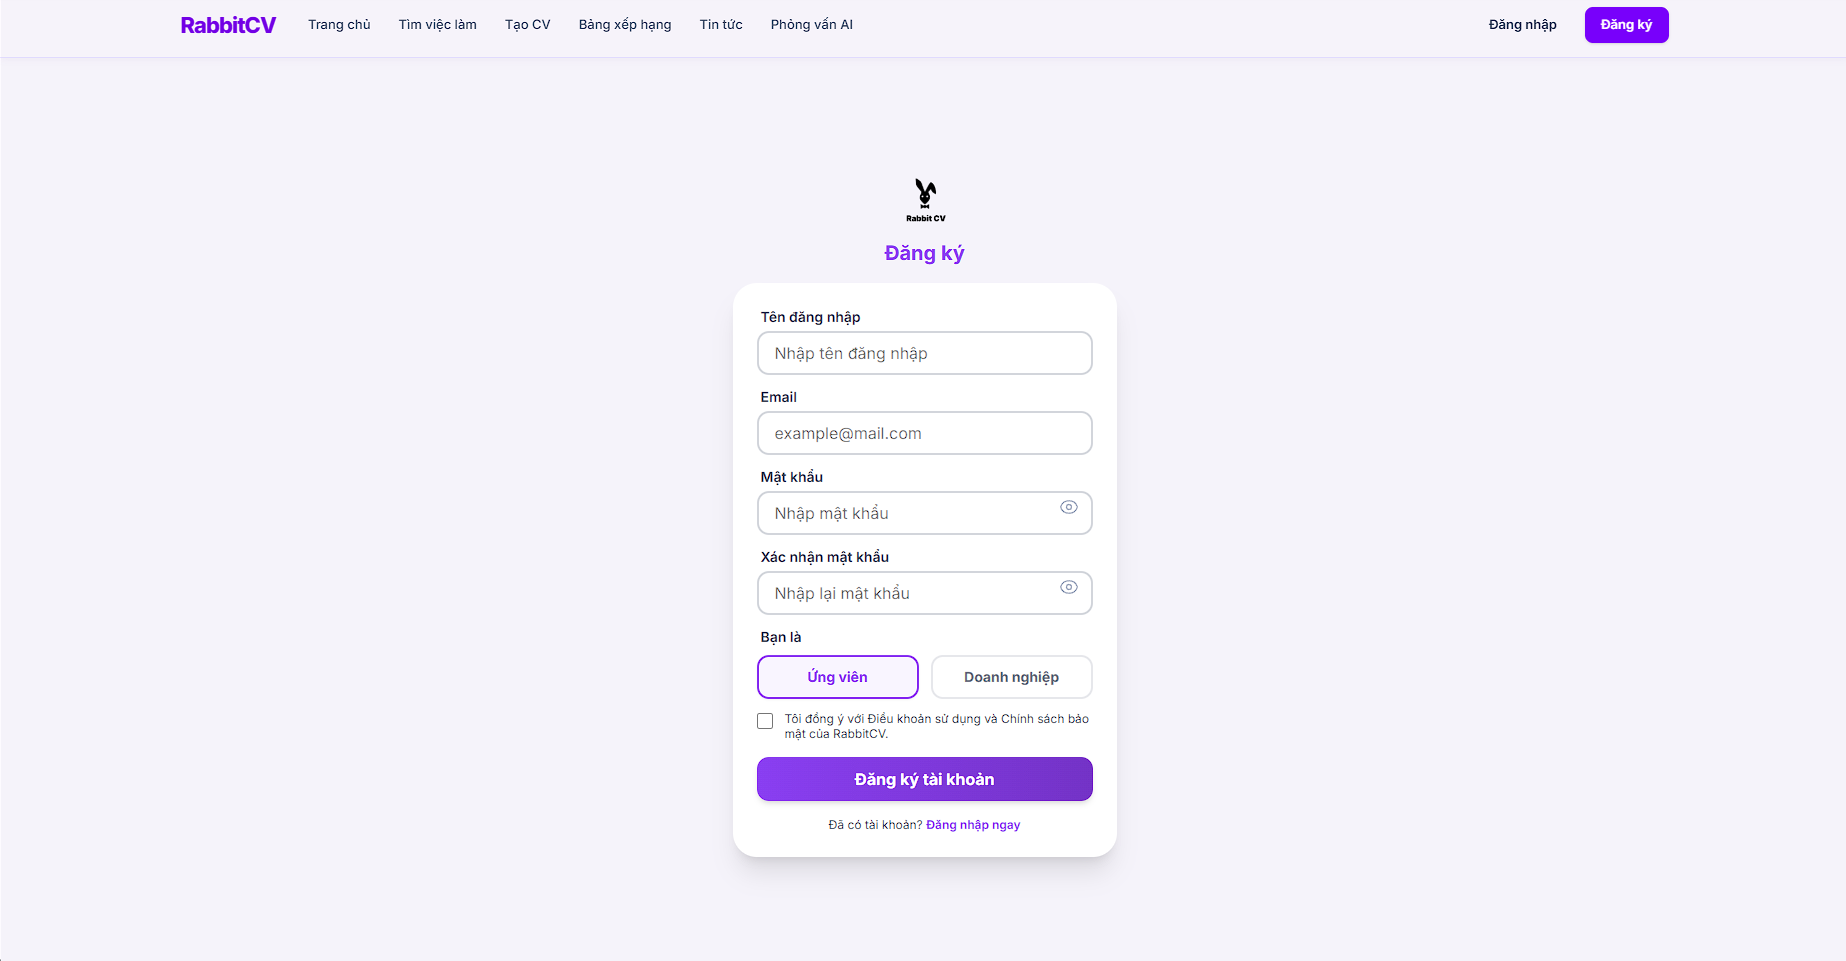
\includegraphics[width=0.87\linewidth,keepaspectratio]{img/Register.png}
    \caption{Giao diện đăng ký tài khoản của RabbitCV}
    \label{fig:register}
\end{figure}

Giao diện đăng ký (Hình~\ref{fig:register}) cho phép người dùng nhập tên đăng nhập, email, mật khẩu, xác nhận mật khẩu và chọn vai trò Ứng viên hoặc Doanh nghiệp. Khi chọn Doanh nghiệp, biểu mẫu yêu cầu thêm tên doanh nghiệp. Người dùng phải đồng ý với điều khoản trước khi gửi yêu cầu. Tài khoản doanh nghiệp tự đăng ký được đưa vào trạng thái chờ quản trị viên phê duyệt trước khi có thể đăng tin tuyển dụng.

Biểu mẫu sử dụng React Hook Form kết hợp Zod để kiểm tra dữ liệu ở frontend và hiển thị lỗi theo trường. Backend tiếp tục kiểm tra thông tin bắt buộc, tên đăng nhập và email trùng, đồng thời băm mật khẩu bằng bcrypt thông qua thư viện bcryptjs trước khi tạo tài khoản. Kiểm tra trên giao diện không thay thế kiểm tra tại máy chủ.

\subsection{Đăng nhập}
\begin{figure}[H]
    \centering
    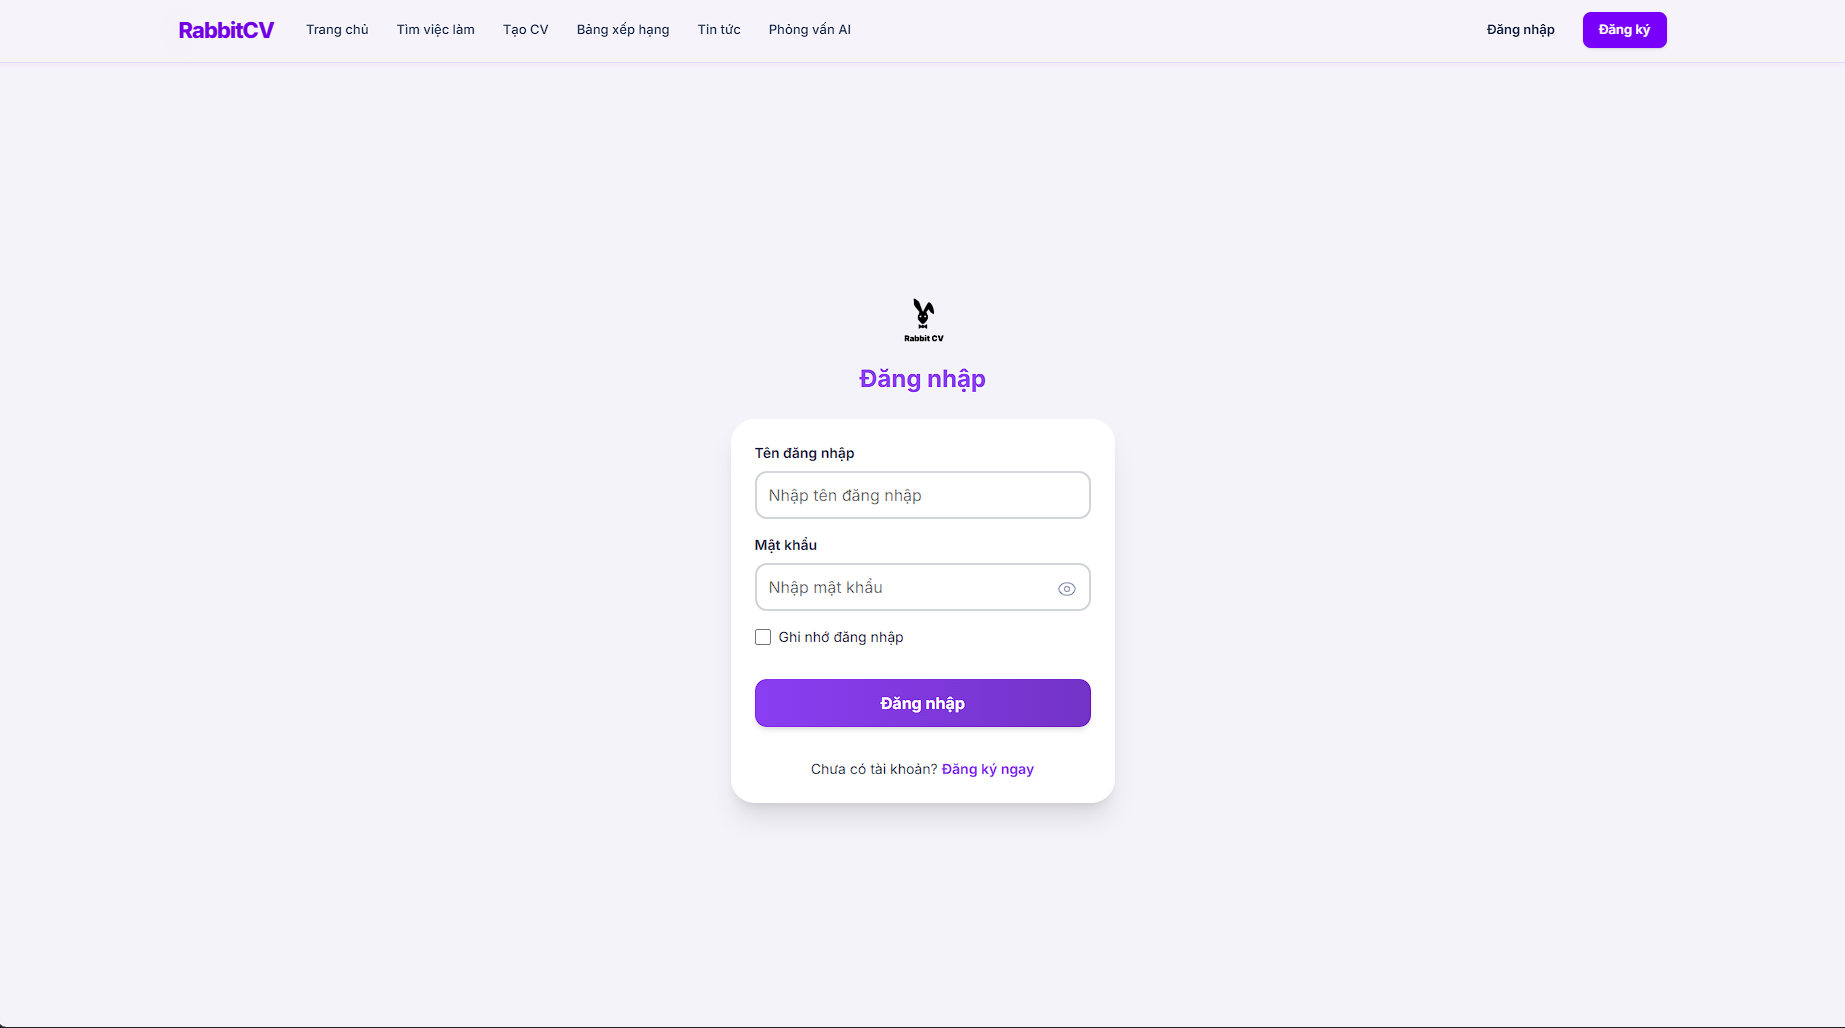
\includegraphics[width=0.87\linewidth,keepaspectratio]{img/Login.png}
    \caption{Giao diện đăng nhập tài khoản của RabbitCV}
    \label{fig:login}
\end{figure}

Giao diện đăng nhập (Hình~\ref{fig:login}) nhận tên đăng nhập hoặc email cùng mật khẩu. Backend kiểm tra tài khoản và mật khẩu, từ chối tài khoản bị khóa hoặc đã bị vô hiệu hóa, sau đó tạo JWT trong cookie HTTP-only nếu xác thực thành công. Tùy chọn \textit{``Ghi nhớ đăng nhập''} thay đổi thời hạn phiên. Giao diện sử dụng thông tin tài khoản để chuyển người dùng đến khu vực ứng viên, doanh nghiệp hoặc quản trị viên.

\subsection{Trang chủ}
\begin{figure}[H]
    \centering
    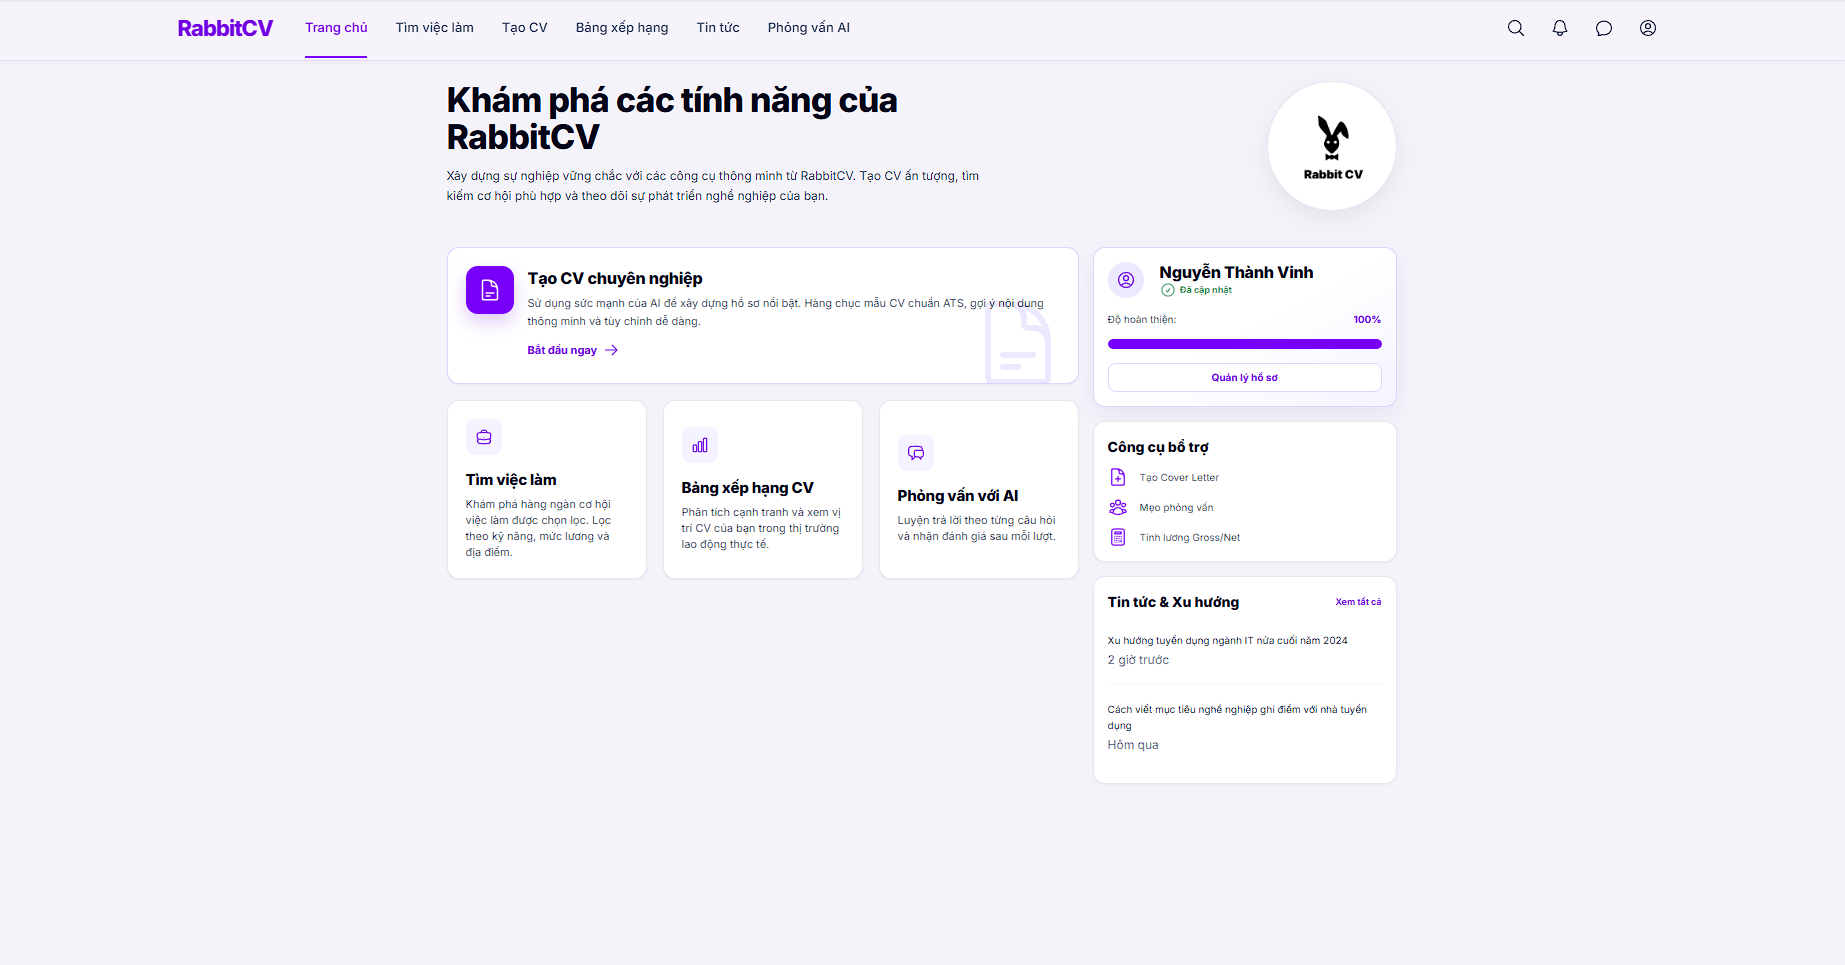
\includegraphics[width=1\linewidth,keepaspectratio]{img/MainMenu.png}
    \caption{Giao diện trang chủ của RabbitCV}
    \label{fig:mainmenu}
\end{figure}

Trang chủ sau khi đăng nhập (Hình~\ref{fig:mainmenu}) đóng vai trò là bảng điều khiển tổng quan dành cho ứng viên. Thanh điều hướng hiển thị các mục chính của hệ thống gồm \textit{Tìm việc làm}, \textit{Bảng xếp hạng CV}, \textit{Phỏng vấn AI} giúp người dùng dễ dàng chuyển đổi qua lại giữa các tính năng. Cột bên phải hiển thị thông tin hồ sơ tóm tắt kèm các liên kết tiện ích hỗ trợ người dùng.

\subsection{Tìm kiếm công việc}

\medskip
\textbf{Trang tìm kiếm công việc}
\medskip

\begin{figure}[H]
    \centering
    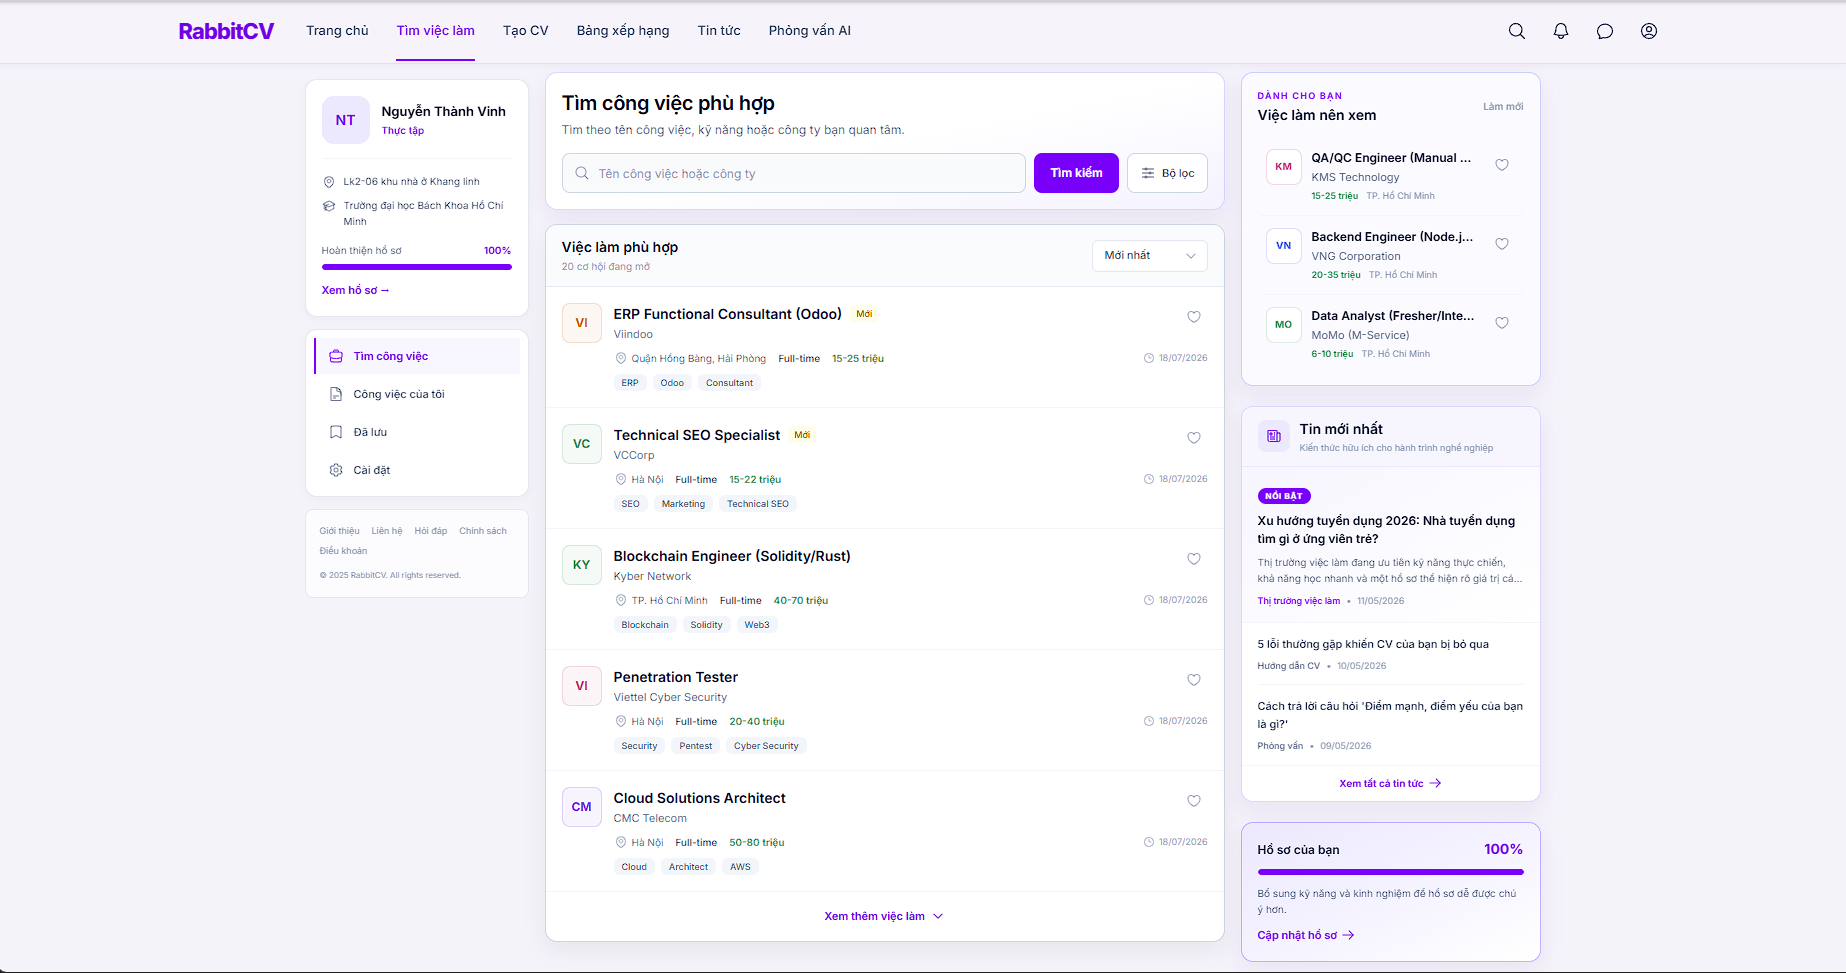
\includegraphics[width=0.95\linewidth,keepaspectratio]{img/Jobs.png}
    \caption{Giao diện tìm kiếm công việc của RabbitCV}
    \label{fig:jobs}
\end{figure}

Trang tìm kiếm việc làm (Hình~\ref{fig:jobs}) cho phép khách và ứng viên tra cứu các tin tuyển dụng công khai theo từ khóa, chức danh hoặc tên công ty, kết hợp bộ lọc và sắp xếp. Mỗi thẻ tin hiển thị tên vị trí, công ty, địa điểm, mức lương và thẻ kỹ năng. Thao tác lưu hoặc bỏ lưu tin yêu cầu đăng nhập; không có kết quả phù hợp được hiển thị bằng danh sách rỗng, không được xem là lỗi hệ thống.

Danh sách việc đã lưu được quản lý trong \texttt{SavedJobsContext} thông qua TanStack Query, với khóa truy vấn theo người dùng. Thao tác lưu hoặc bỏ lưu cập nhật cache trước để phản hồi trên giao diện; nếu API thất bại thì khôi phục dữ liệu cũ và hiển thị lỗi, sau đó truy vấn lại để đồng bộ với máy chủ.

\medskip
\textbf{Trang chi tiết công việc}
\medskip

\begin{figure}[H]
    \centering
    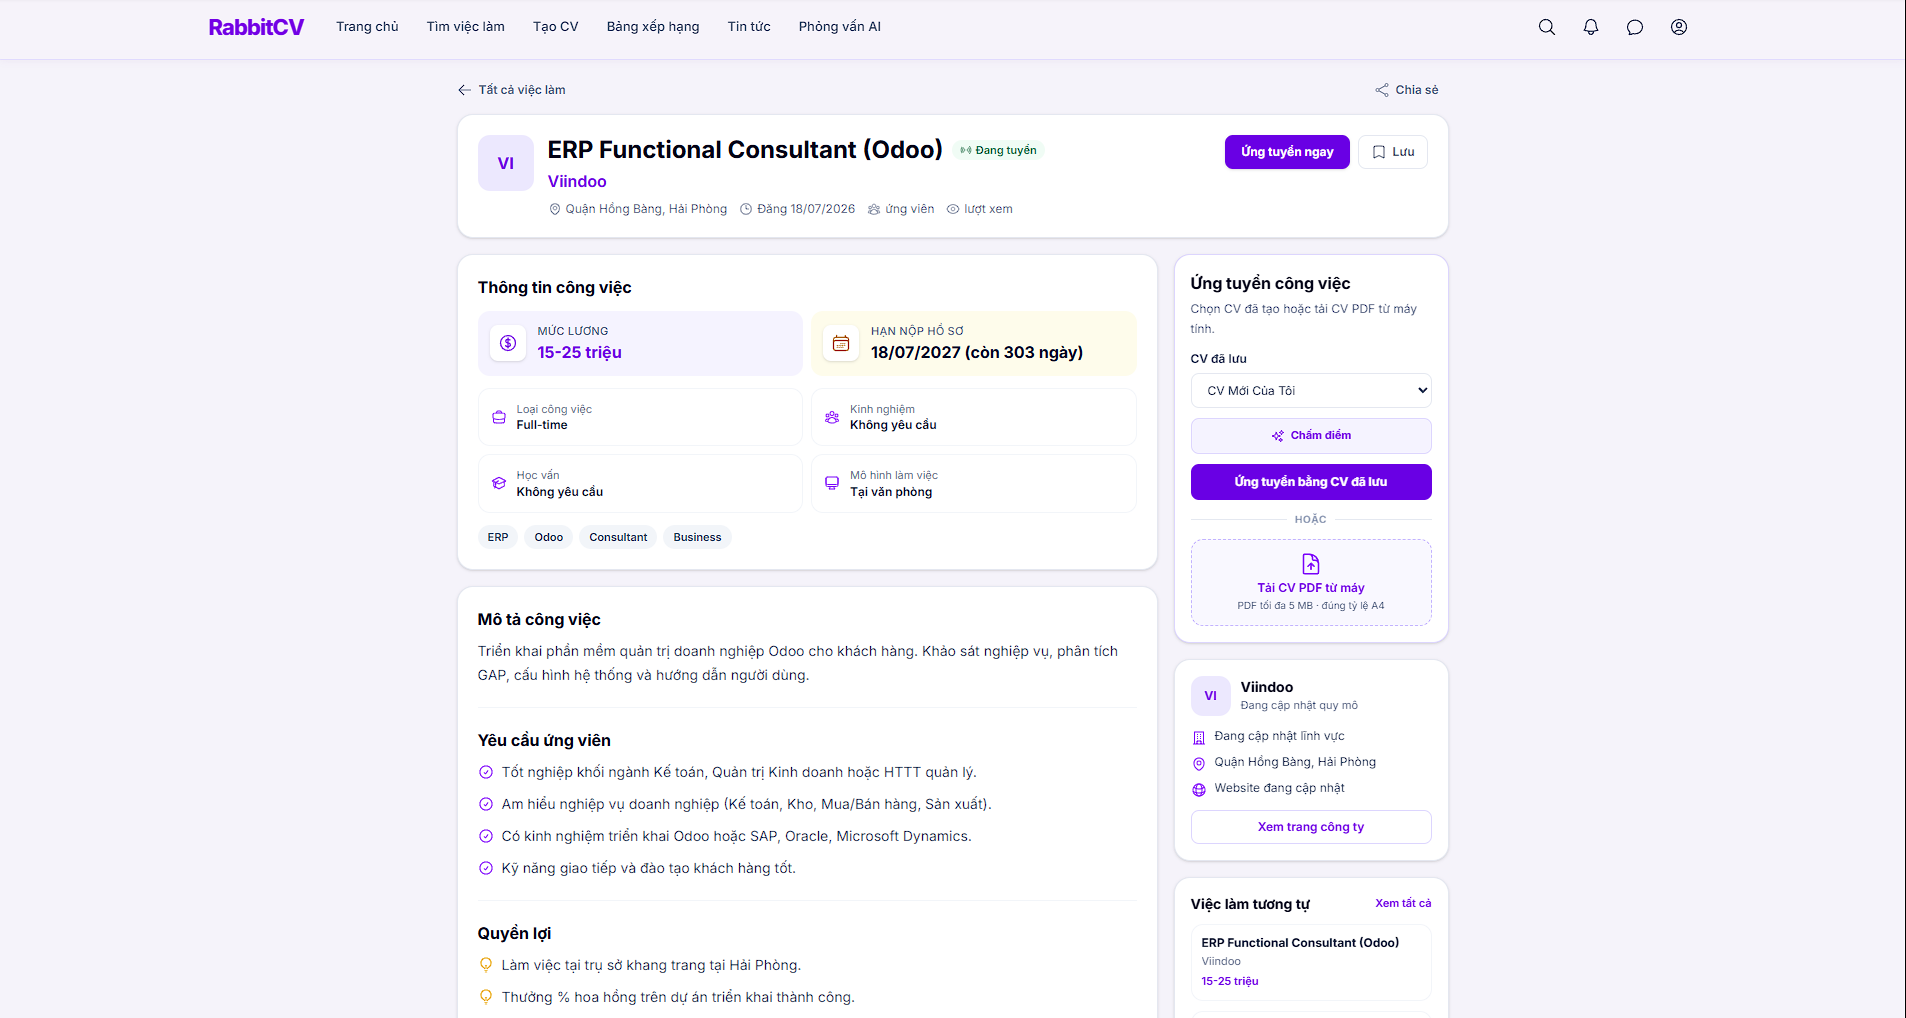
\includegraphics[width=0.95\linewidth,keepaspectratio]{img/JobDetail.png}
    \caption{Giao diện chi tiết công việc của RabbitCV}
    \label{fig:jobdetail}
\end{figure}

Trang chi tiết công việc (Hình~\ref{fig:jobdetail}) cung cấp đầy đủ thông tin về vị trí tuyển dụng gồm mức lương, hạn nộp, mô tả công việc, yêu cầu và quyền lợi ứng viên. Cột bên phải tích hợp khung ứng tuyển cho phép nộp hồ sơ bằng CV đã lưu hoặc tải lên tệp PDF từ máy tính. Ngoài ra, người dùng có thể lưu lại tin tuyển dụng hoặc bắt đầu trò chuyện trực tiếp để trao đổi với doanh nghiệp.

\clearpage
\textbf{Lựa chọn CV để ứng tuyển}
\medskip

\begin{figure}[H]
    \centering
    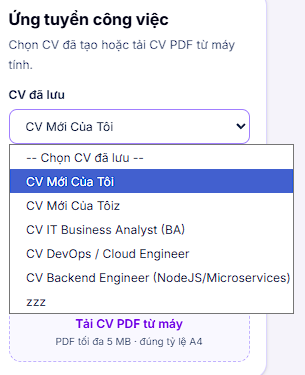
\includegraphics[width=0.3\linewidth,keepaspectratio]{img/CVSelectionApply.png}
    \caption{Giao diện lựa chọn CV để ứng tuyển của RabbitCV}
    \label{fig:cvselectionapply}
\end{figure}

Hộp thoại lựa chọn CV (Hình~\ref{fig:cvselectionapply}) cho phép ứng viên chọn CV đã lưu hoặc tệp CV PDF từ thiết bị trước khi xác nhận ứng tuyển. PDF tải lên phải đáp ứng điều kiện định dạng và có dung lượng không vượt quá 5~MB. Bộ kiểm tra hiện tại không xác minh khổ giấy A4 của tệp tải lên.

Hai cách nộp hồ sơ được tiếp nhận qua các API ứng tuyển tương ứng. Backend kiểm tra tin còn nhận hồ sơ, quyền sở hữu CV khi chọn bản đã lưu và việc ứng tuyển trùng. Hồ sơ mới được tạo trong \texttt{Application} với trạng thái "Chờ duyệt", kèm \texttt{jobSnapshot} và \texttt{resumeSnapshot}. Bản chụp này giữ nội dung đã nộp độc lập với những lần sửa CV sau đó; chỉ mục duy nhất trên cặp tin tuyển dụng và ứng viên bổ sung ràng buộc chống nộp trùng.

\subsection{Quản lý CV}

\medskip
\textbf{Trang danh sách CV}
\medskip

\begin{figure}[H]
    \centering
    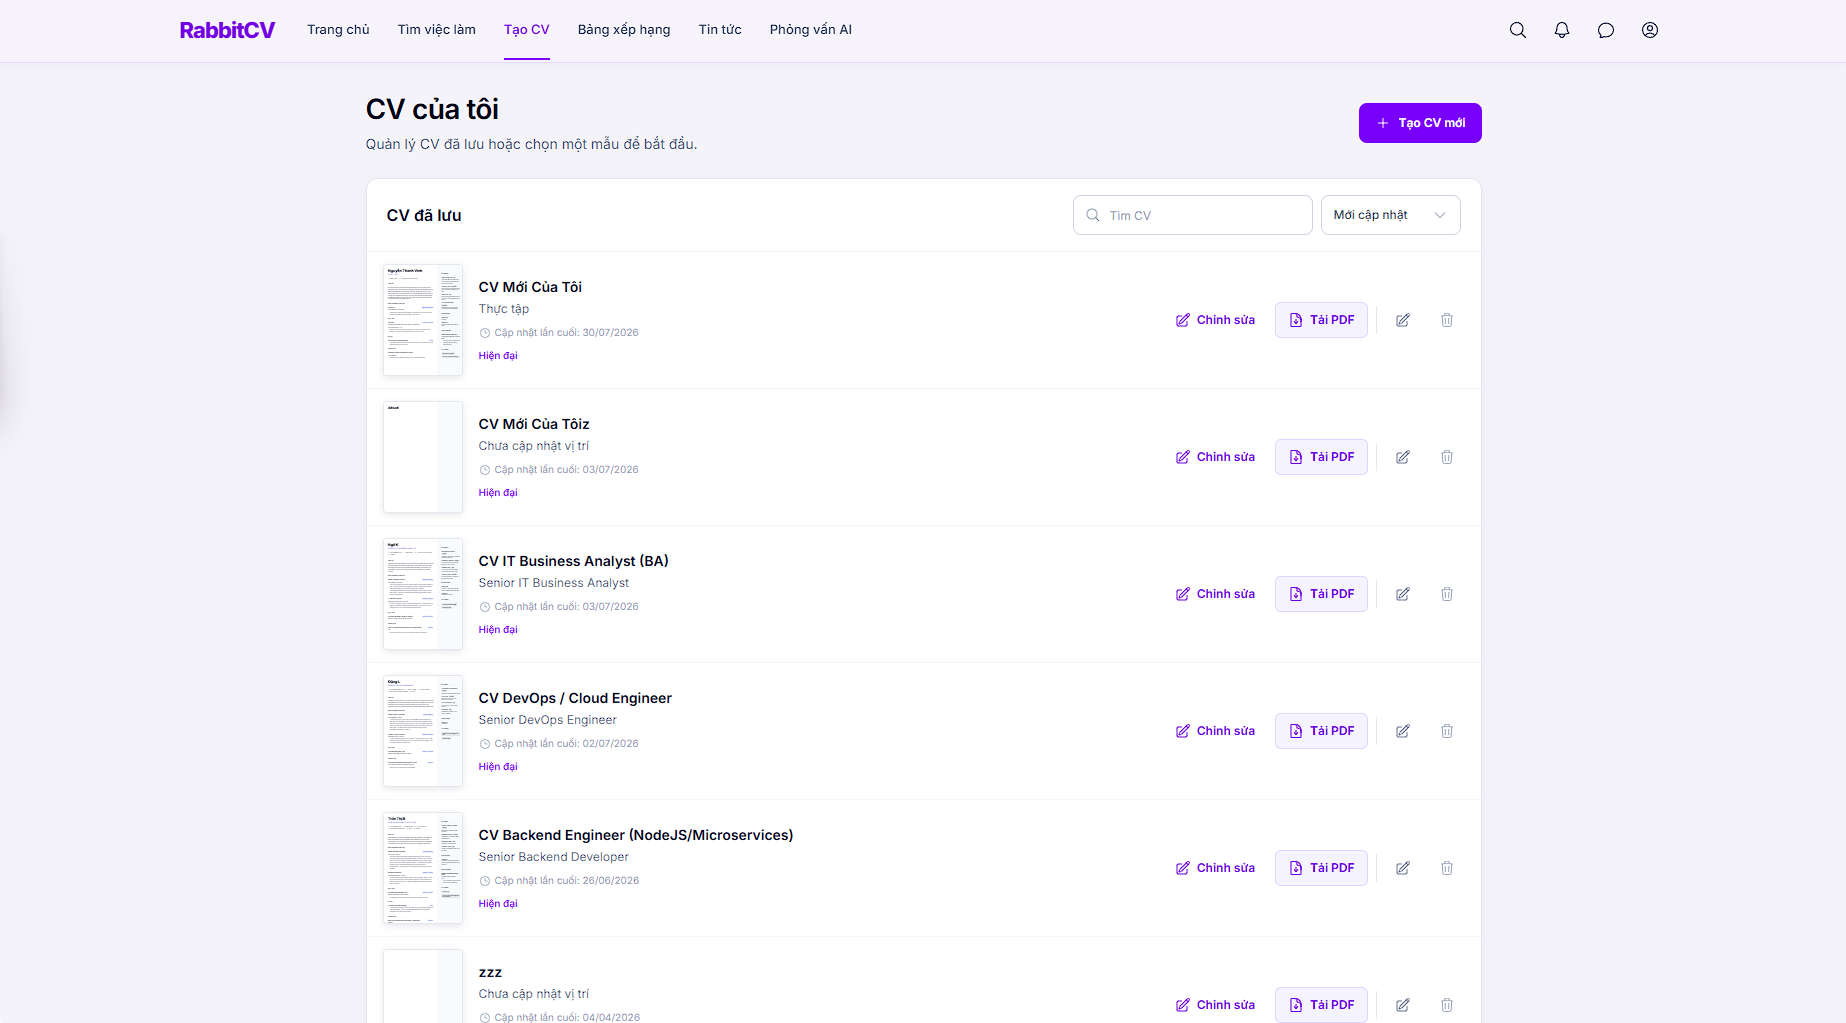
\includegraphics[width=0.95\linewidth,keepaspectratio]{img/CVs.png}
    \caption{Giao diện danh sách CV của RabbitCV}
    \label{fig:cvs}
\end{figure}

Trang quản lý danh sách CV (Hình~\ref{fig:cvs}) hiển thị các CV thuộc người dùng với tên, vị trí mục tiêu, thời gian cập nhật và mẫu trình bày. Các thao tác gồm tạo mới, chỉnh sửa, xuất PDF, đổi tên và xóa. API danh sách loại trường \texttt{pdfData} khỏi kết quả phản hồi và không đưa các CV tạm tạo khi ứng tuyển bằng PDF vào danh sách quản lý thông thường.

Đối với CV có cấu trúc, chức năng xuất sử dụng hook \texttt{useResumePrint} để mở hộp thoại in của trình duyệt với cấu hình trang A4. Người dùng chọn lưu thành PDF hoặc hủy thao tác. Đây không phải luồng backend tạo rồi gửi một tệp PDF, và việc mở hoặc đóng hộp thoại in không chứng minh người dùng đã lưu tệp thành công.

\medskip
\textbf{Trang chỉnh sửa CV}
\medskip

\begin{figure}[H]
    \centering
    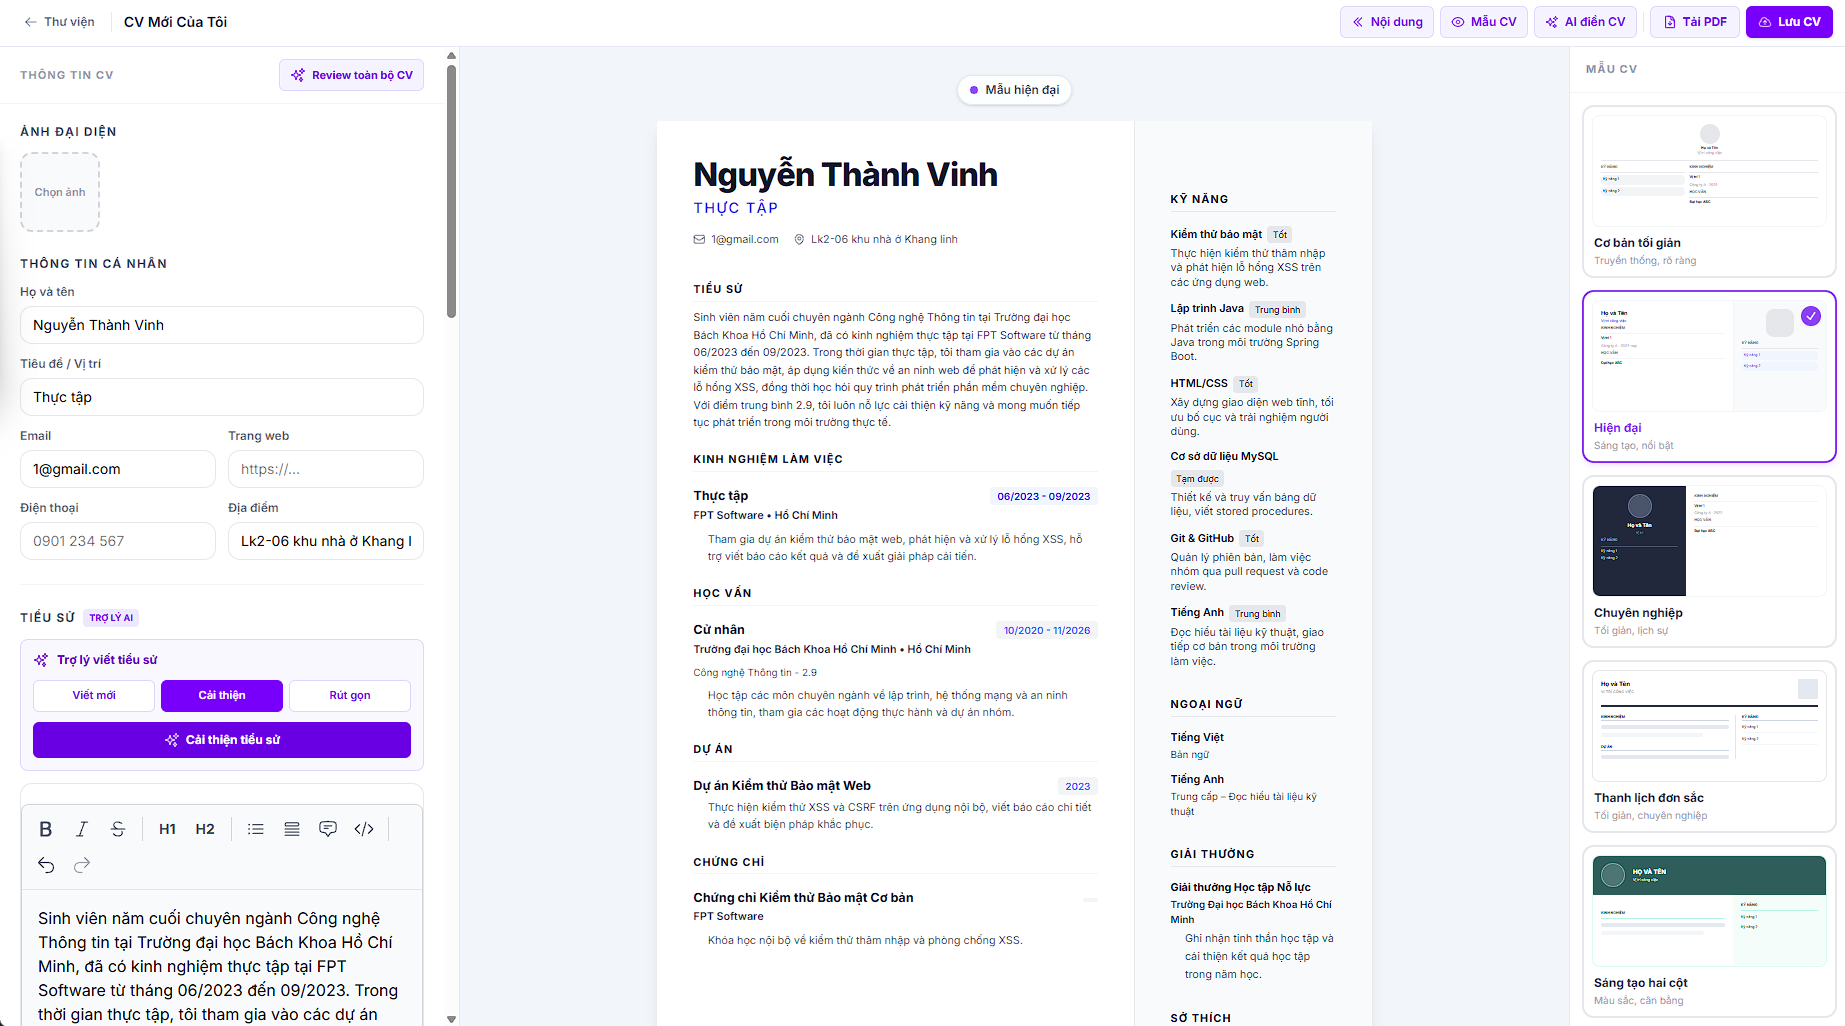
\includegraphics[width=0.98\linewidth,keepaspectratio]{img/CV_Edit.png}
    \caption{Trang chỉnh sửa nội dung CV của RabbitCV}
    \label{fig:cvedit}
\end{figure}

Trang chỉnh sửa CV (Hình~\ref{fig:cvedit}) là nơi ứng viên xây dựng và hoàn thiện nội dung hồ sơ. Giao diện được chia thành ba khu vực chuyên biệt:

\begin{itemize}
    \item \textbf{Khu vực điền nội dung}: Chứa thông tin cá nhân, tiểu sử, kinh nghiệm, học vấn, kỹ năng, dự án, chứng chỉ và các nhóm nội dung tùy chỉnh. Người dùng thêm, sửa hoặc bỏ nội dung theo nhu cầu; có thể yêu cầu AI rà soát CV và gợi ý bổ sung phần còn thiếu. Không có chức năng AI viết lại nội dung riêng biệt trong phiên bản hiện tại.
    \item \textbf{Khu vực xem trước CV}: Cập nhật trực tiếp dữ liệu đang chỉnh sửa và hiển thị nội dung theo chuẩn khổ in A4. Khu vực này tích hợp cơ chế kéo-thả (\textit{Drag-and-Drop}) linh hoạt, cho phép người dùng nhấp giữ và sắp xếp lại vị trí các khối nội dung giữa các cột và vùng bố cục theo ý muốn.
    \item \textbf{Khu vực lựa chọn mẫu}: Cung cấp các mẫu giao diện CV được thiết kế sẵn. Hệ thống tự động cập nhật phong cách và bố cục ngay khi người dùng chuyển đổi sang một mẫu CV mới.
\end{itemize}

Trang soạn thảo giữ dữ liệu đang chỉnh sửa trong trạng thái React, còn \texttt{ResumePreview} dựng bản xem trước từ dữ liệu đó. Hook \texttt{useResumeHistory} cung cấp cơ chế hoàn tác (\textit{Undo}) và làm lại (\textit{Redo}) đa cấp cho cả thao tác nhập liệu văn bản lẫn thao tác kéo-thả sắp xếp bố cục. Thay đổi, bao gồm gợi ý AI được bổ sung, chỉ được ghi vào cơ sở dữ liệu khi người dùng nhấn Lưu; việc cập nhật bản xem trước không phải thao tác lưu tự động.

\subsection{Trang bảng xếp hạng}

\begin{figure}[H]
    \centering
    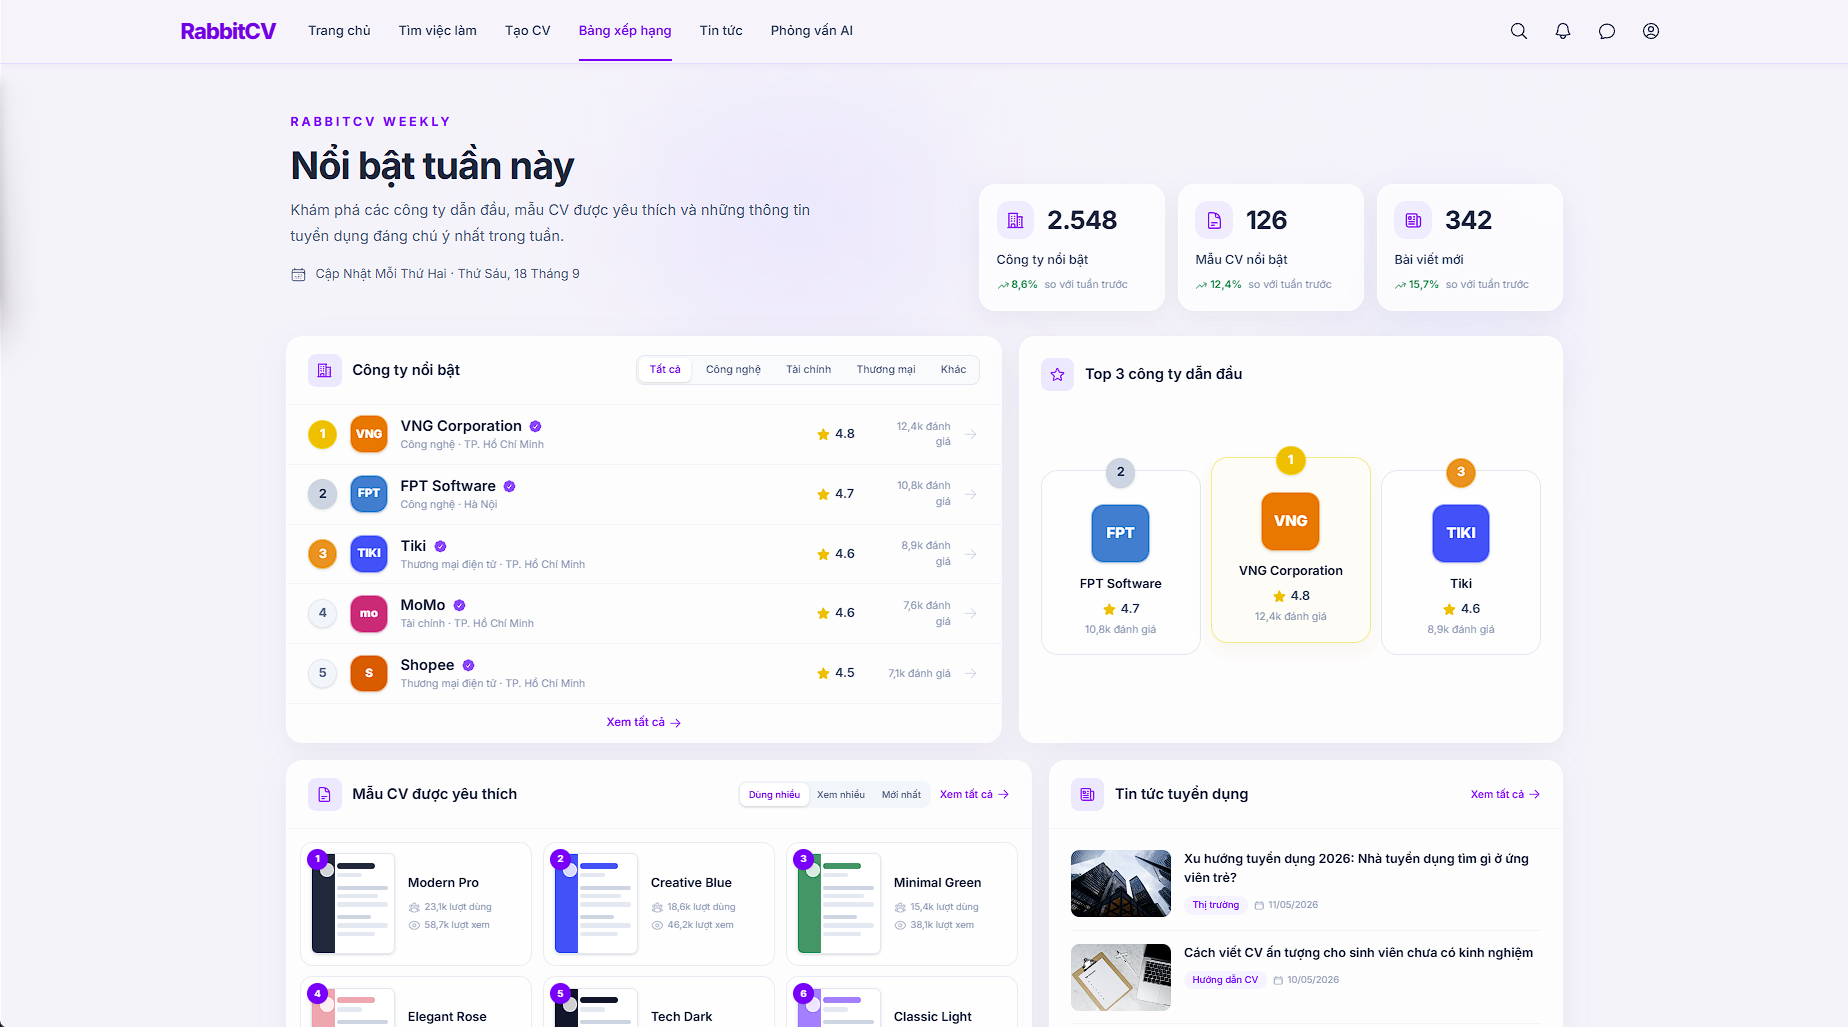
\includegraphics[width=0.95\linewidth,keepaspectratio]{img/TopPage.png}
    \caption{Trang bảng xếp hạng của RabbitCV}
    \label{fig:cvtop}
\end{figure}

Trang bảng xếp hạng (Hình~\ref{fig:cvtop}) minh họa cách trình bày doanh nghiệp nổi bật và mẫu CV được quan tâm. Trong phiên bản hiện tại, các chỉ số tổng quan, điểm sao doanh nghiệp, lượt xem và lượt sử dụng mẫu CV được khai báo bằng dữ liệu mẫu ở frontend. Vì vậy, những số liệu này chỉ phục vụ trình diễn giao diện, không phải thống kê hằng tuần được tổng hợp từ hoạt động thực tế của người dùng.

\subsection{Trang tin tức}

\medskip
\textbf{Trang danh sách tin tức}
\medskip

\begin{figure}[H]
    \centering
    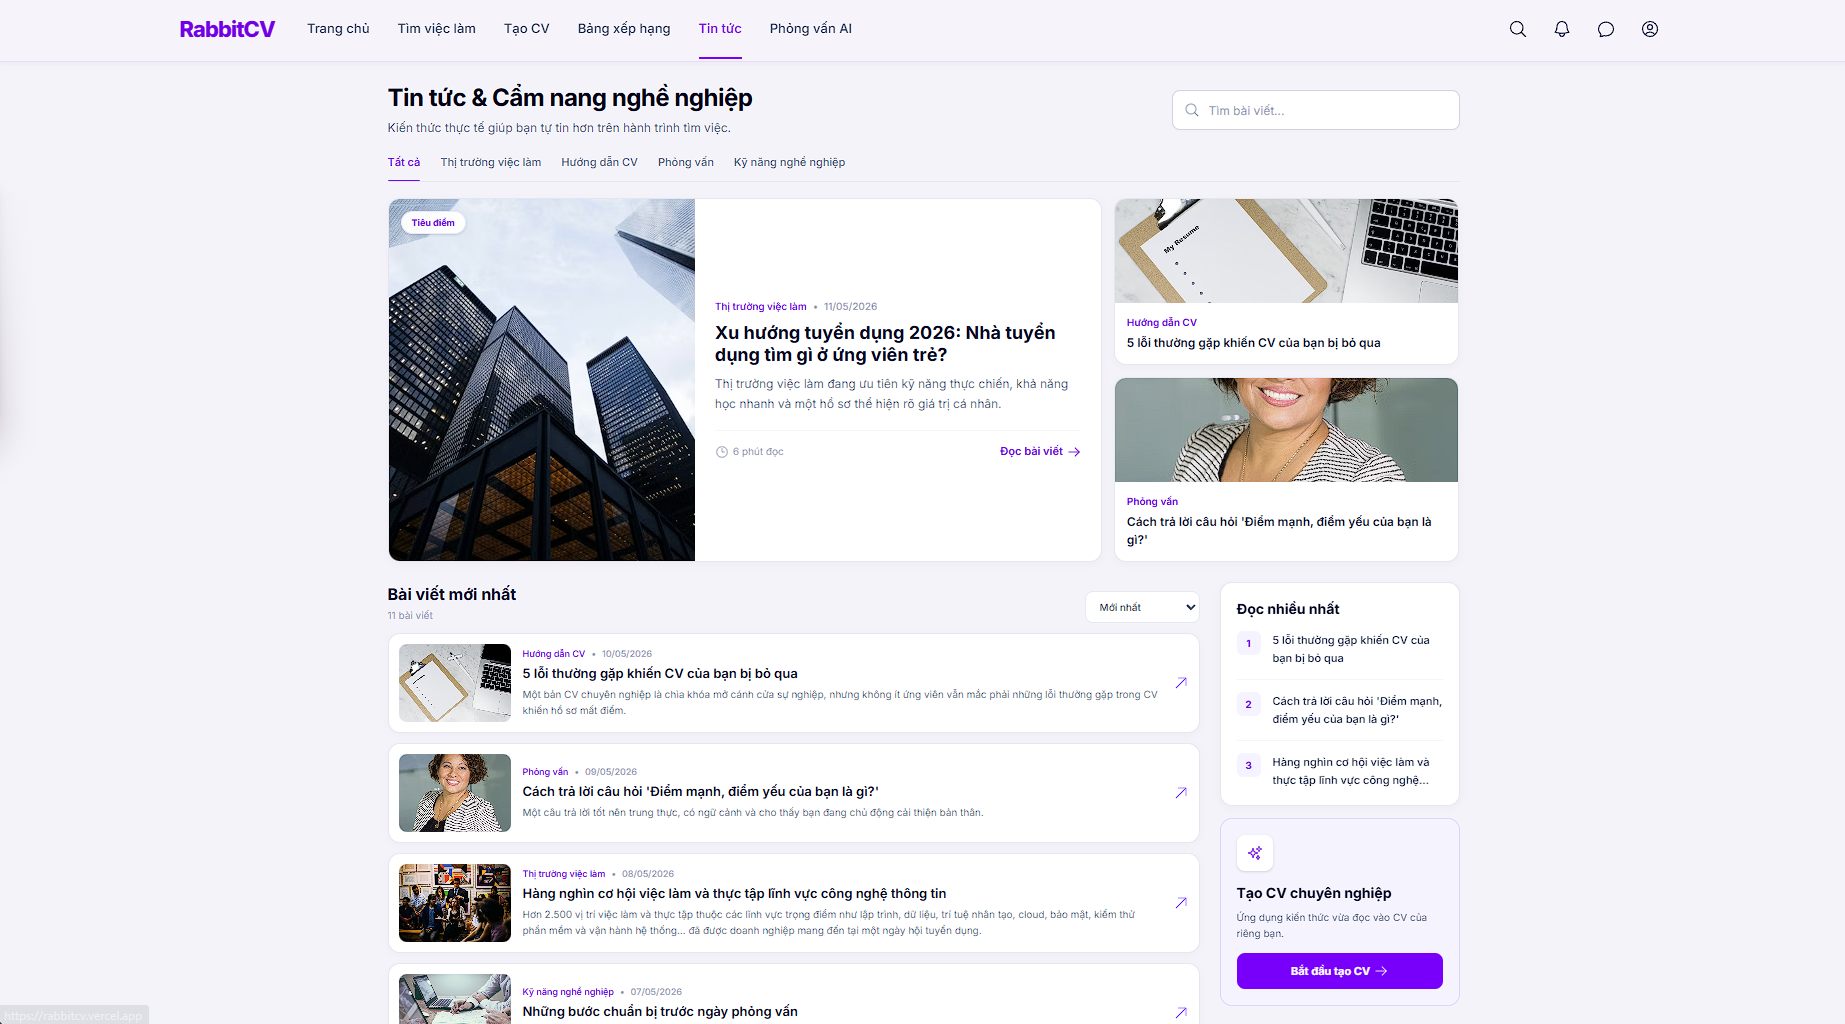
\includegraphics[width=0.9\linewidth,keepaspectratio]{img/NewsPage.png}
    \caption{Trang tin tức của RabbitCV}
    \label{fig:news}
\end{figure}

Trang tin tức (Hình~\ref{fig:news}) hiển thị các bài viết về thị trường việc làm, viết CV, phỏng vấn và phát triển nghề nghiệp. Giao diện tổ chức nội dung thành các nhóm bài viết và cho phép lựa chọn theo danh mục. Hook \texttt{usePublicNews} lấy danh sách từ API tin tức và quản lý cache bằng TanStack Query, đồng thời truy vấn lại để cập nhật nội dung.

\medskip
\textbf{Trang chi tiết tin tức}
\medskip

\begin{figure}[H]
    \centering
    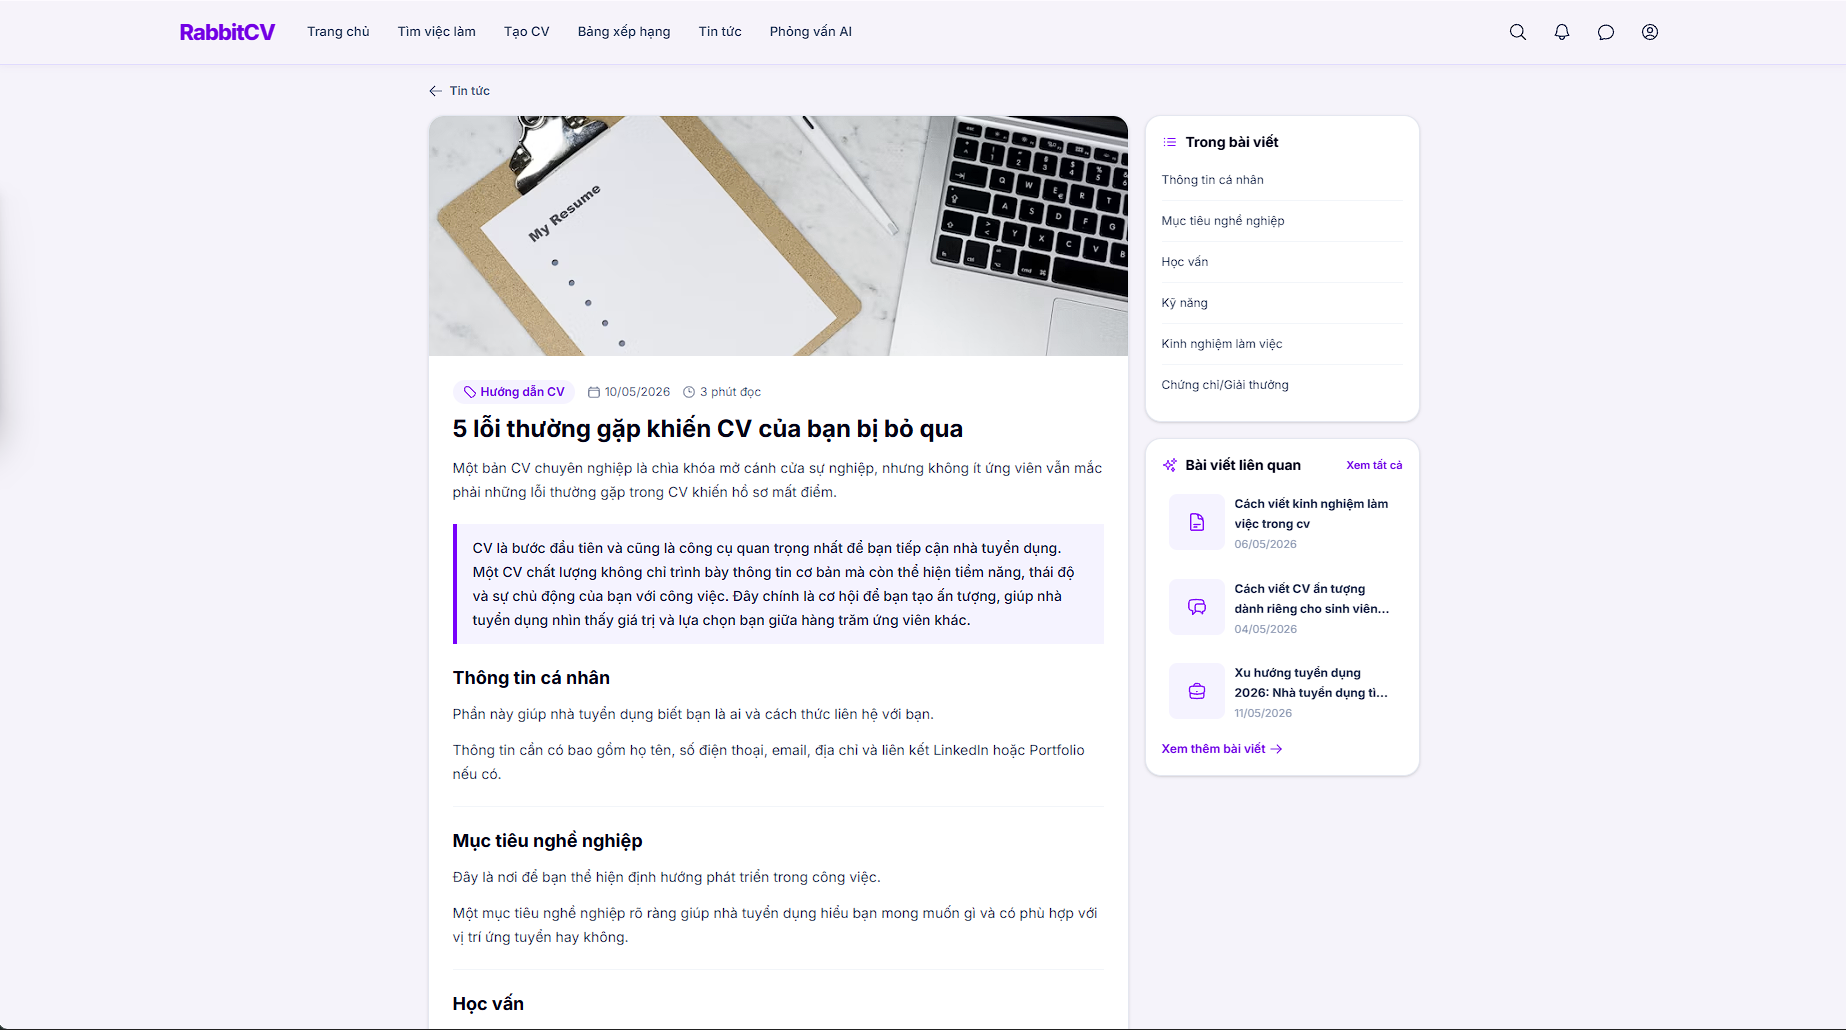
\includegraphics[width=1\linewidth,keepaspectratio]{img/NewsDetail.png}
    \caption{Trang chi tiết tin tức của RabbitCV}
    \label{fig:newsdetail}
\end{figure}

Trang chi tiết bài viết (Hình~\ref{fig:newsdetail}) được thiết kế tối ưu cho trải nghiệm đọc: hiển thị hình ảnh đại diện, tiêu đề bài viết, thời gian đọc ước tính, nội dung phân đoạn mạch lạc kèm trích dẫn nổi bật; đồng thời tích hợp thanh mục lục điều hướng nhanh và danh sách bài viết liên quan ở cột bên phải.


\clearpage
\subsection{Phỏng vấn AI}

\textbf{Trang phỏng vấn với AI}
\medskip
\begin{figure}[H]
    \centering
    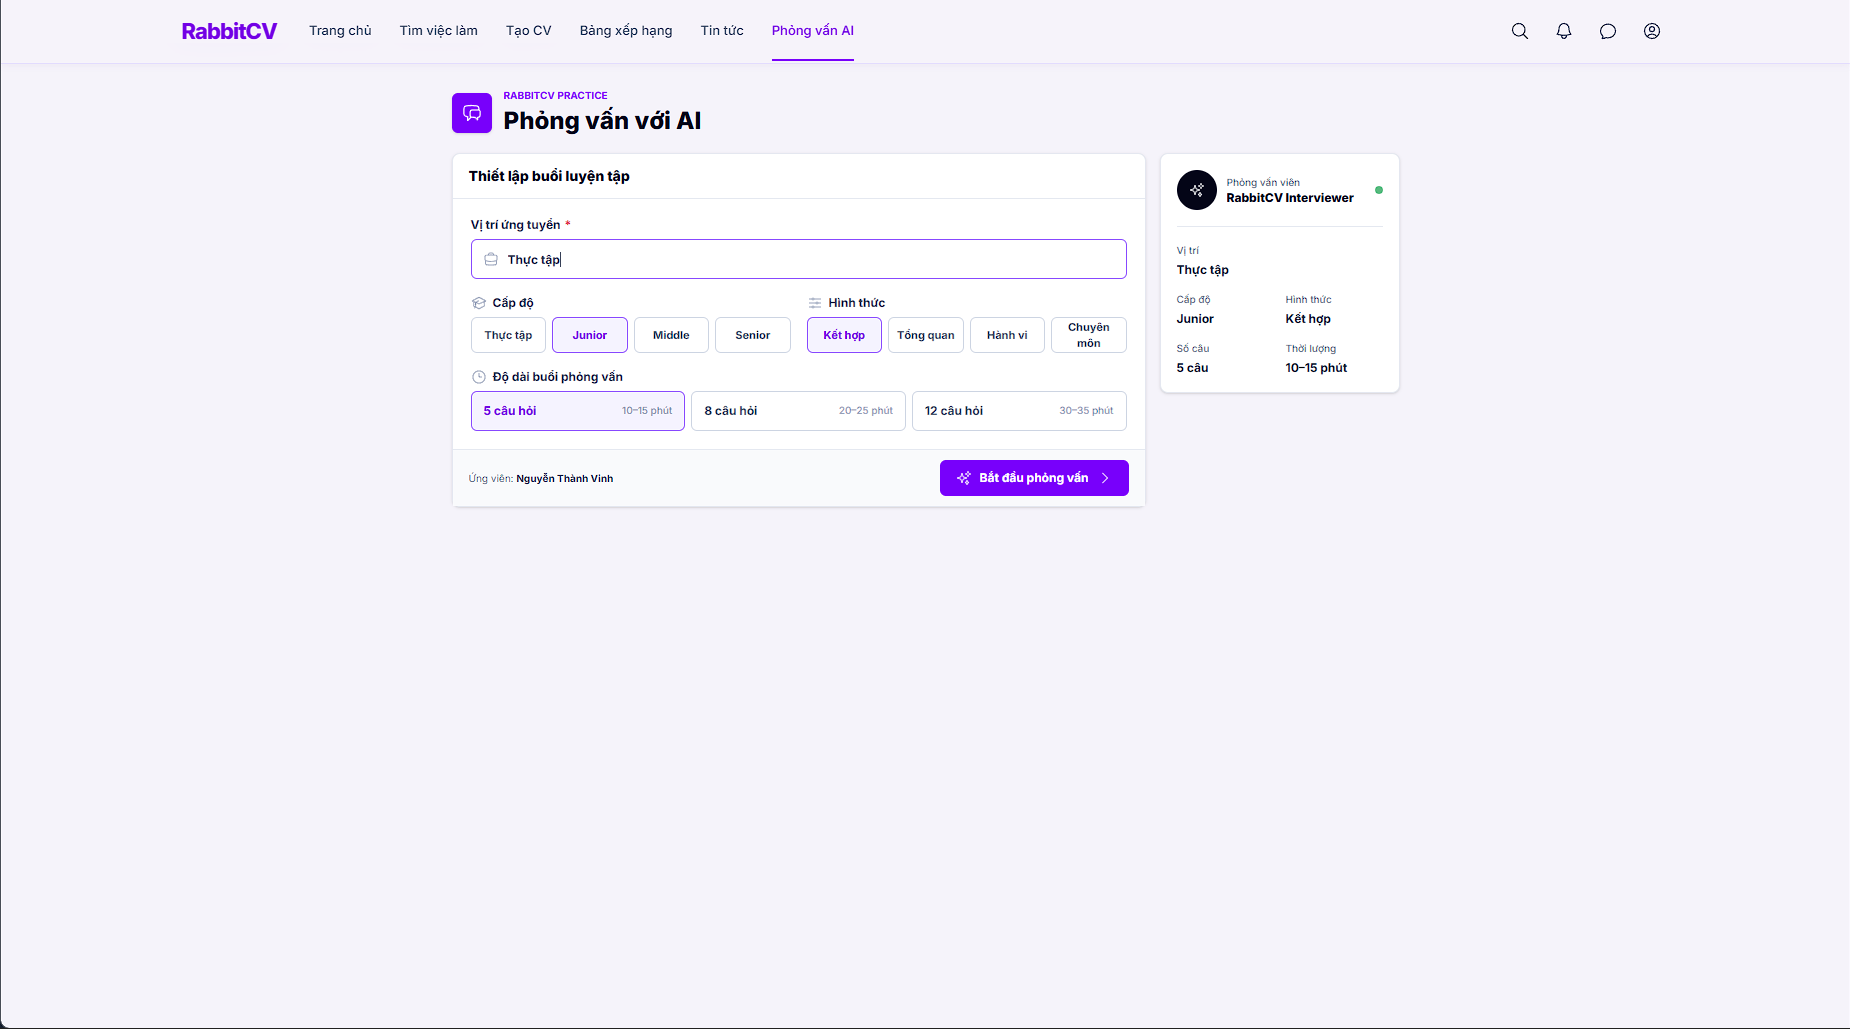
\includegraphics[width=1\linewidth,keepaspectratio]{img/AIInterview.png}
    \caption{Trang phỏng vấn AI của RabbitCV}
    \label{fig:aiinterview}
\end{figure}

Trang phỏng vấn AI (Hình~\ref{fig:aiinterview}) cung cấp không gian luyện tập phỏng vấn thử thông minh dành cho ứng viên. Tại đây, ứng viên có thể lựa chọn vị trí công việc mục tiêu, cấp độ chuyên môn, hình thức phỏng vấn và số lượng câu hỏi mong muốn trước khi bắt đầu phiên phỏng vấn.


\medskip
\textbf{Trang nhắn tin phỏng vấn}
\medskip

\begin{figure}[H]
    \centering
    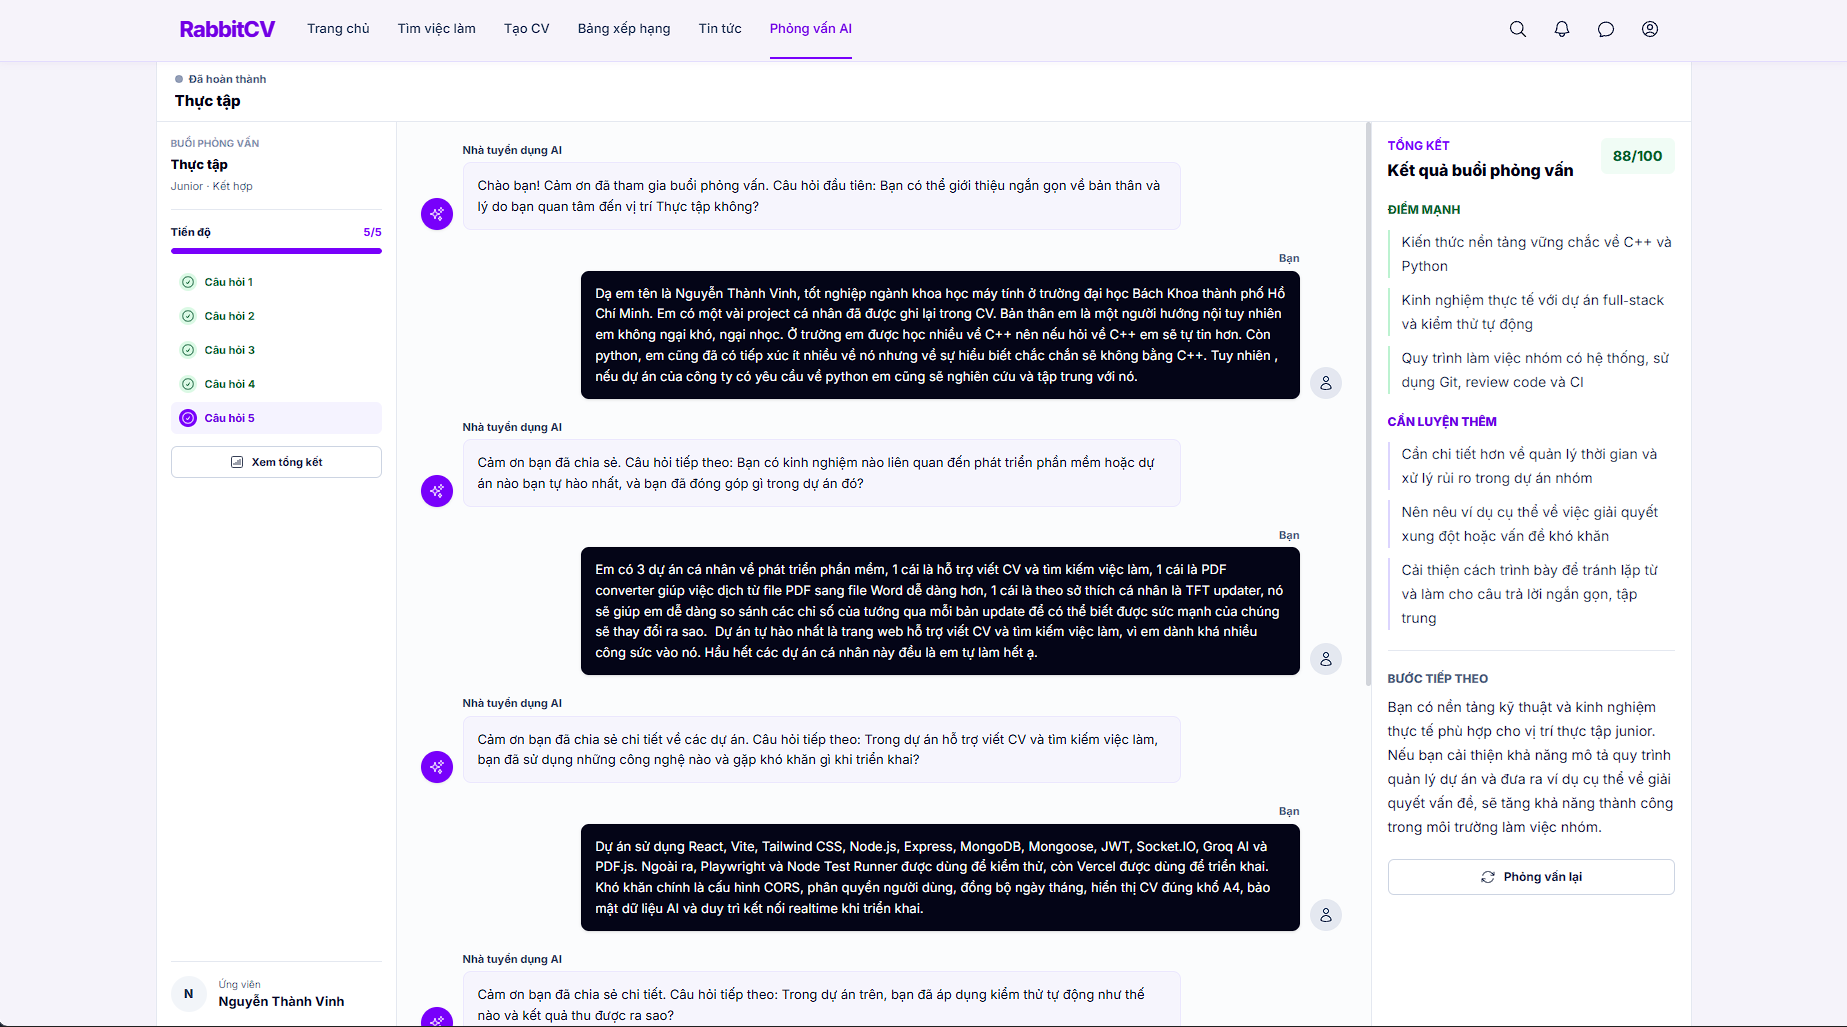
\includegraphics[width=1\linewidth,keepaspectratio]{img/AIInterviewChat.png}
    \caption{Trang nhắn tin phỏng vấn của RabbitCV}
    \label{fig:aiinterviewchat}
\end{figure}

Giao diện nhắn tin phỏng vấn (Hình~\ref{fig:aiinterviewchat}) hiển thị câu hỏi của AI, câu trả lời của ứng viên và nhận xét theo từng lượt. Trang gửi yêu cầu HTTP đến API phỏng vấn và hiển thị trạng thái chờ trong thời gian xử lý, không sử dụng Socket.IO để nhận câu trả lời AI. Khi hoàn tất, người dùng xem phần tổng kết hoặc chọn \textit{``Phỏng vấn lại''} để bắt đầu phiên mới. Điểm nhận xét chỉ phục vụ luyện tập; lịch sử phiên chưa được lưu vào cơ sở dữ liệu và sẽ mất khi tải lại trang. Chi tiết xử lý được trình bày tại Chương~\ref{chap:ai-module}.

\subsection{Trang cá nhân}


\begin{figure}[H]
    \centering
    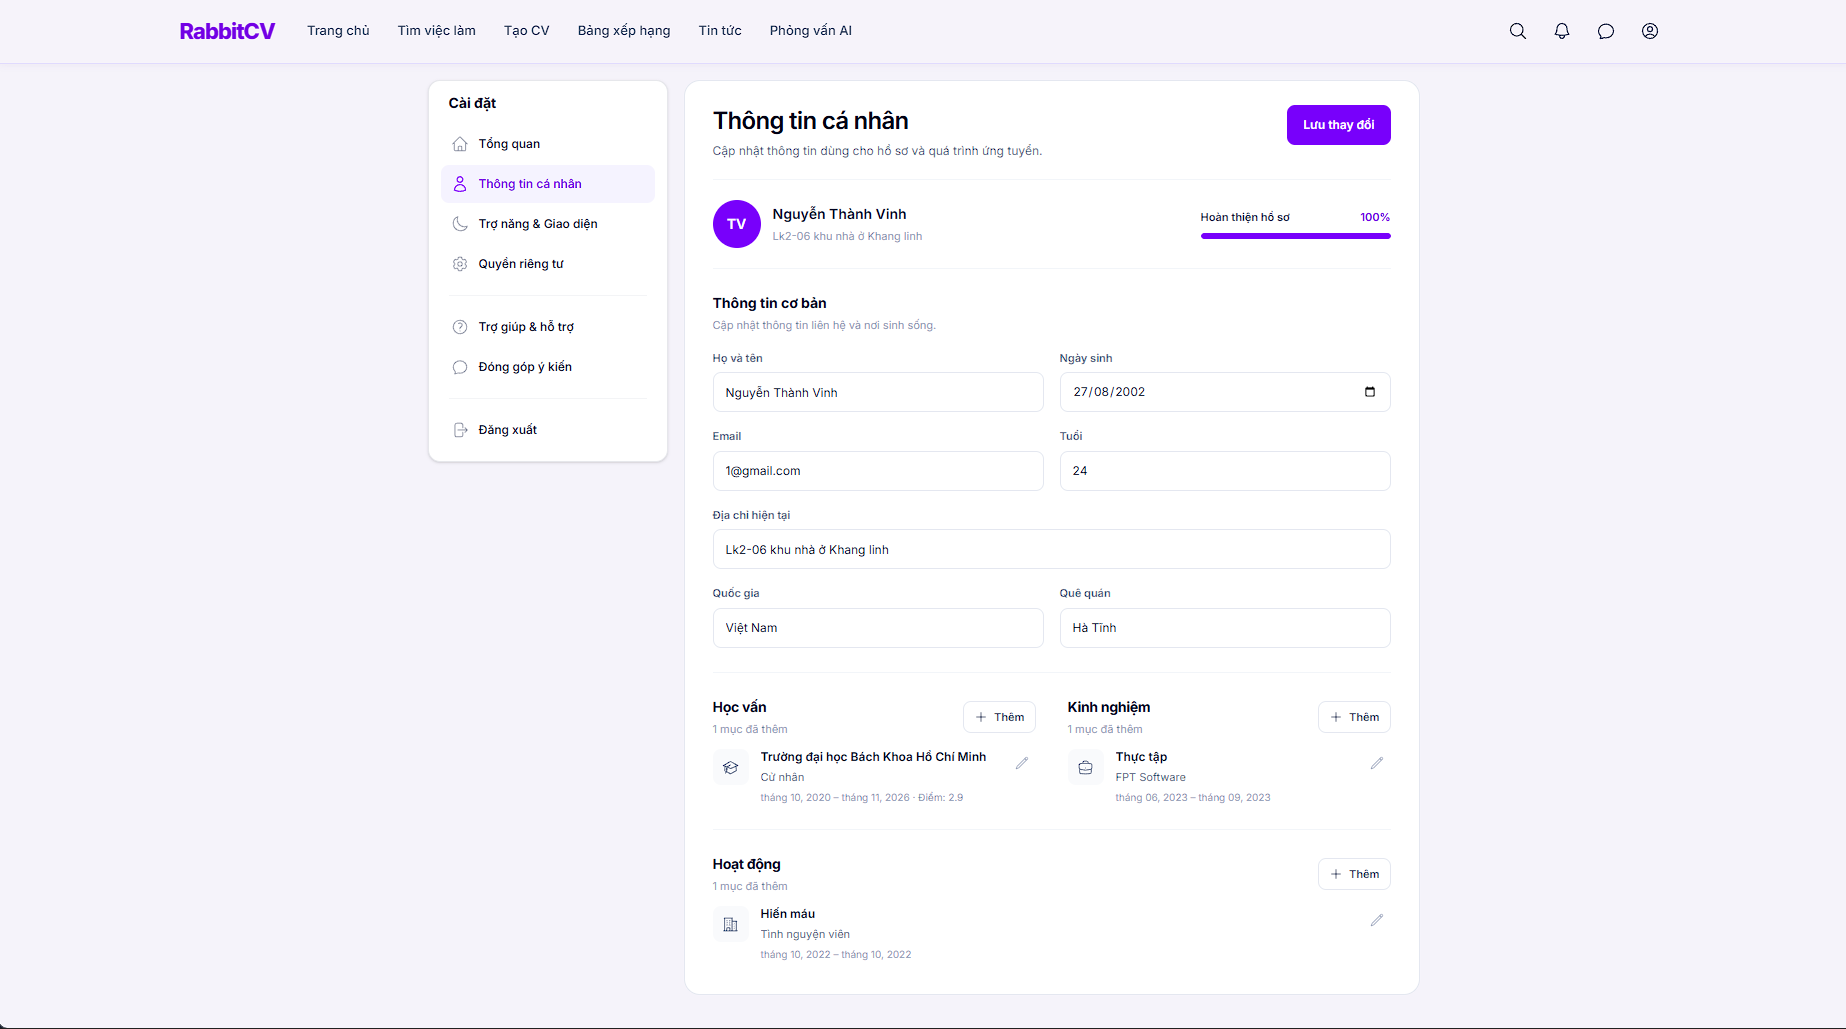
\includegraphics[width=1\linewidth,keepaspectratio]{img/Profile.png}
    \caption{Trang cá nhân của RabbitCV}
    \label{fig:profile}
\end{figure}

Trang cá nhân (Hình~\ref{fig:profile}) là nơi ứng viên quản lý thông tin tài khoản và thiết lập hồ sơ ứng tuyển chuyên nghiệp. Giao diện bao gồm menu cài đặt ở cột bên trái và khu vực cập nhật chi tiết ở bên phải, cho phép ứng viên theo dõi mức độ hoàn thiện hồ sơ, chỉnh sửa thông tin liên hệ cơ bản, đồng thời thêm mới hoặc cập nhật các mục học vấn, kinh nghiệm làm việc và hoạt động tham gia.

\section{Doanh nghiệp}

\subsection{Trang tổng quan}

\begin{figure}[H]
    \centering
    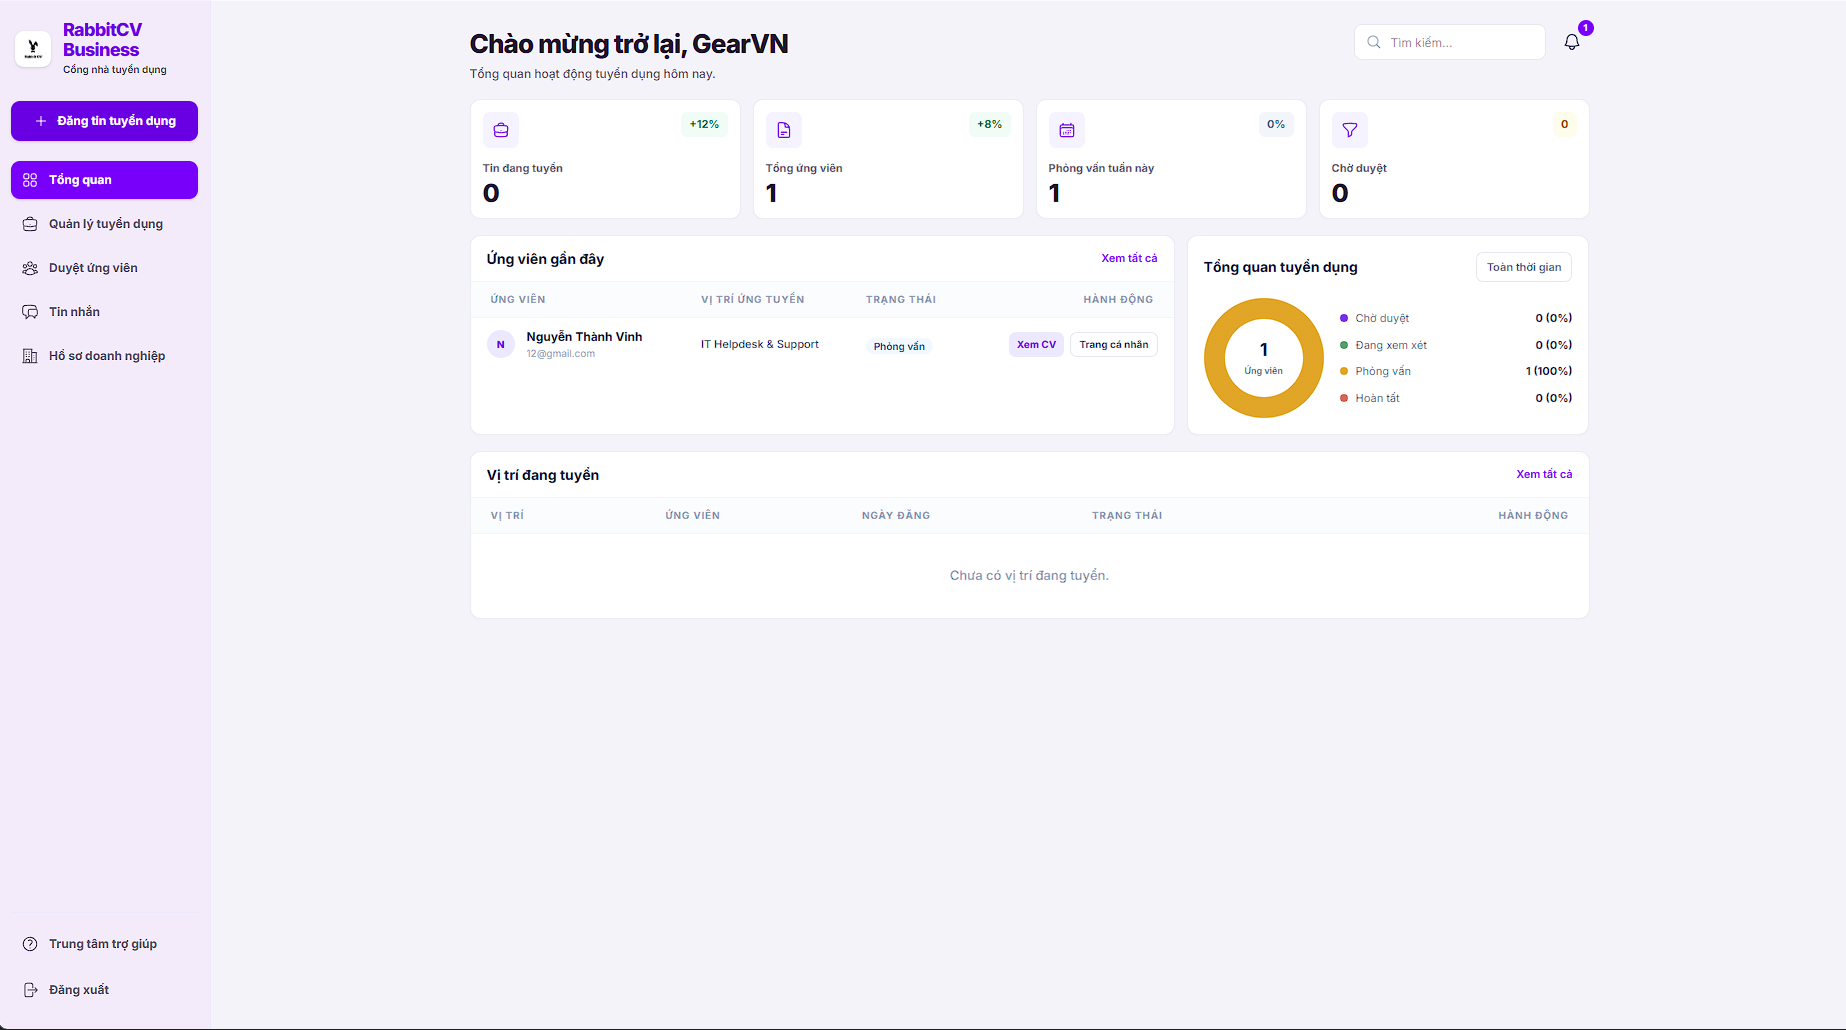
\includegraphics[width=0.95\linewidth,keepaspectratio]{img/CompanyOverview.png}
    \caption{Giao diện tổng quan của doanh nghiệp}
    \label{fig:companyoverview}
\end{figure}

Trang tổng quan (Hình~\ref{fig:companyoverview}) tổng hợp tin tuyển dụng và hồ sơ thuộc doanh nghiệp đang đăng nhập. Các chỉ số gồm số tin đang tuyển, tổng số hồ sơ ứng tuyển, số hồ sơ ở trạng thái phỏng vấn và số hồ sơ chờ duyệt. Biểu đồ thể hiện phân bố trạng thái hồ sơ; danh sách gần đây hỗ trợ mở CV hoặc hồ sơ ứng viên.

Các chỉ số được tính từ danh sách tin và hồ sơ tải về. Chỉ số phỏng vấn hiện đếm các hồ sơ có trạng thái \texttt{Interview}, không lọc theo ngày hẹn hoặc theo tuần. Vì vậy, dù nhãn giao diện còn ghi \textit{``Phỏng vấn tuần này''}, dữ liệu này chưa thể được xem là lịch phỏng vấn trong tuần.

\subsection{Hồ sơ doanh nghiệp}

\begin{figure}[H]
    \centering
    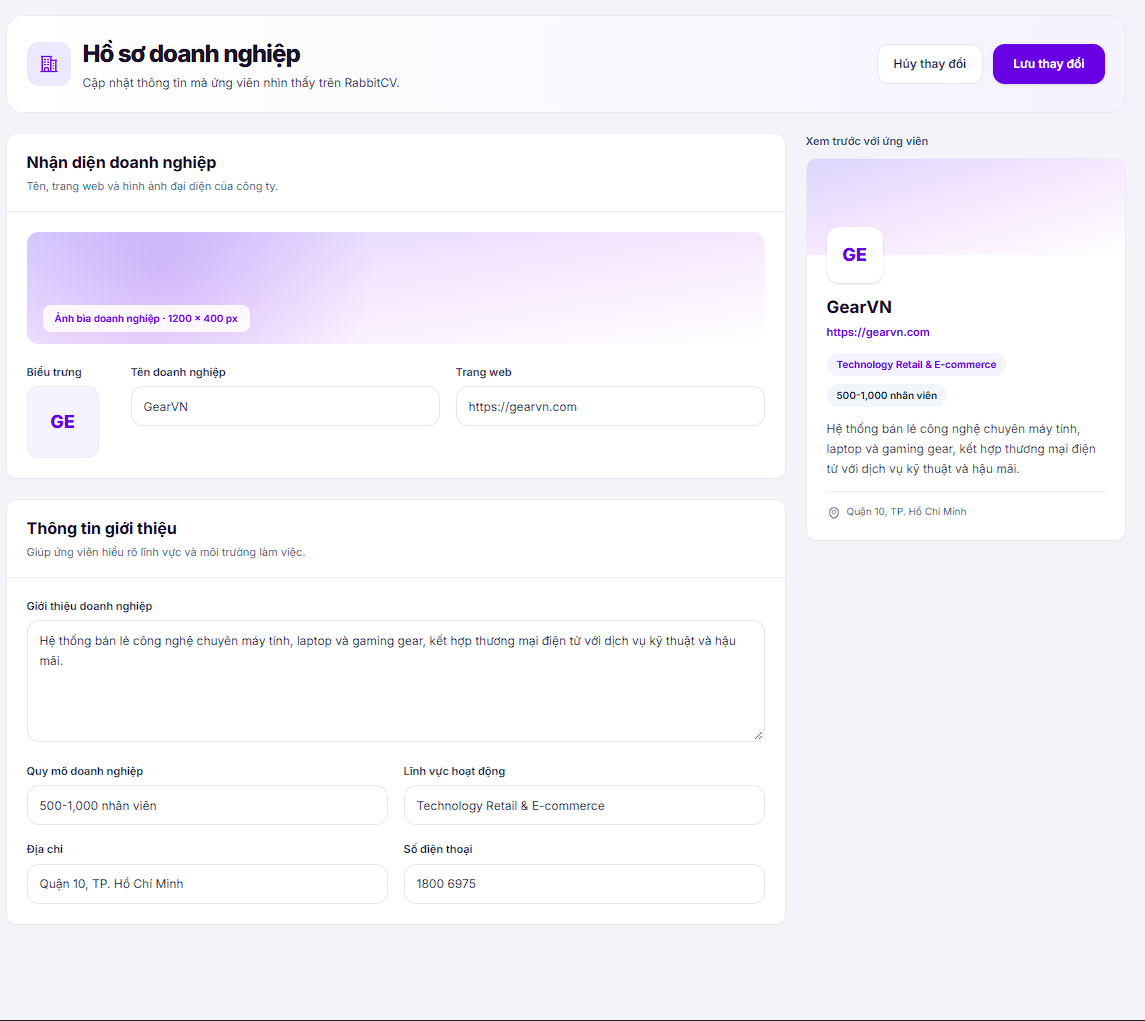
\includegraphics[width=1\linewidth,keepaspectratio]{img/CompanyProfile.png}
    \caption{Giao diện quản lý hồ sơ doanh nghiệp}
    \label{fig:companyprofile}
\end{figure}

Trang hồ sơ doanh nghiệp (Hình~\ref{fig:companyprofile}) cho phép cập nhật ảnh bìa, biểu trưng, tên công ty, website, quy mô, lĩnh vực hoạt động, địa chỉ và giới thiệu. Khung xem trước cập nhật theo dữ liệu biểu mẫu để người dùng kiểm tra trước khi lưu. Thay đổi trên bản xem trước chưa phải dữ liệu đã được lưu; hồ sơ chỉ được cập nhật tại máy chủ sau khi thao tác lưu thành công.

\subsection{Đăng tin tuyển dụng}

\begin{figure}[H]
    \centering
    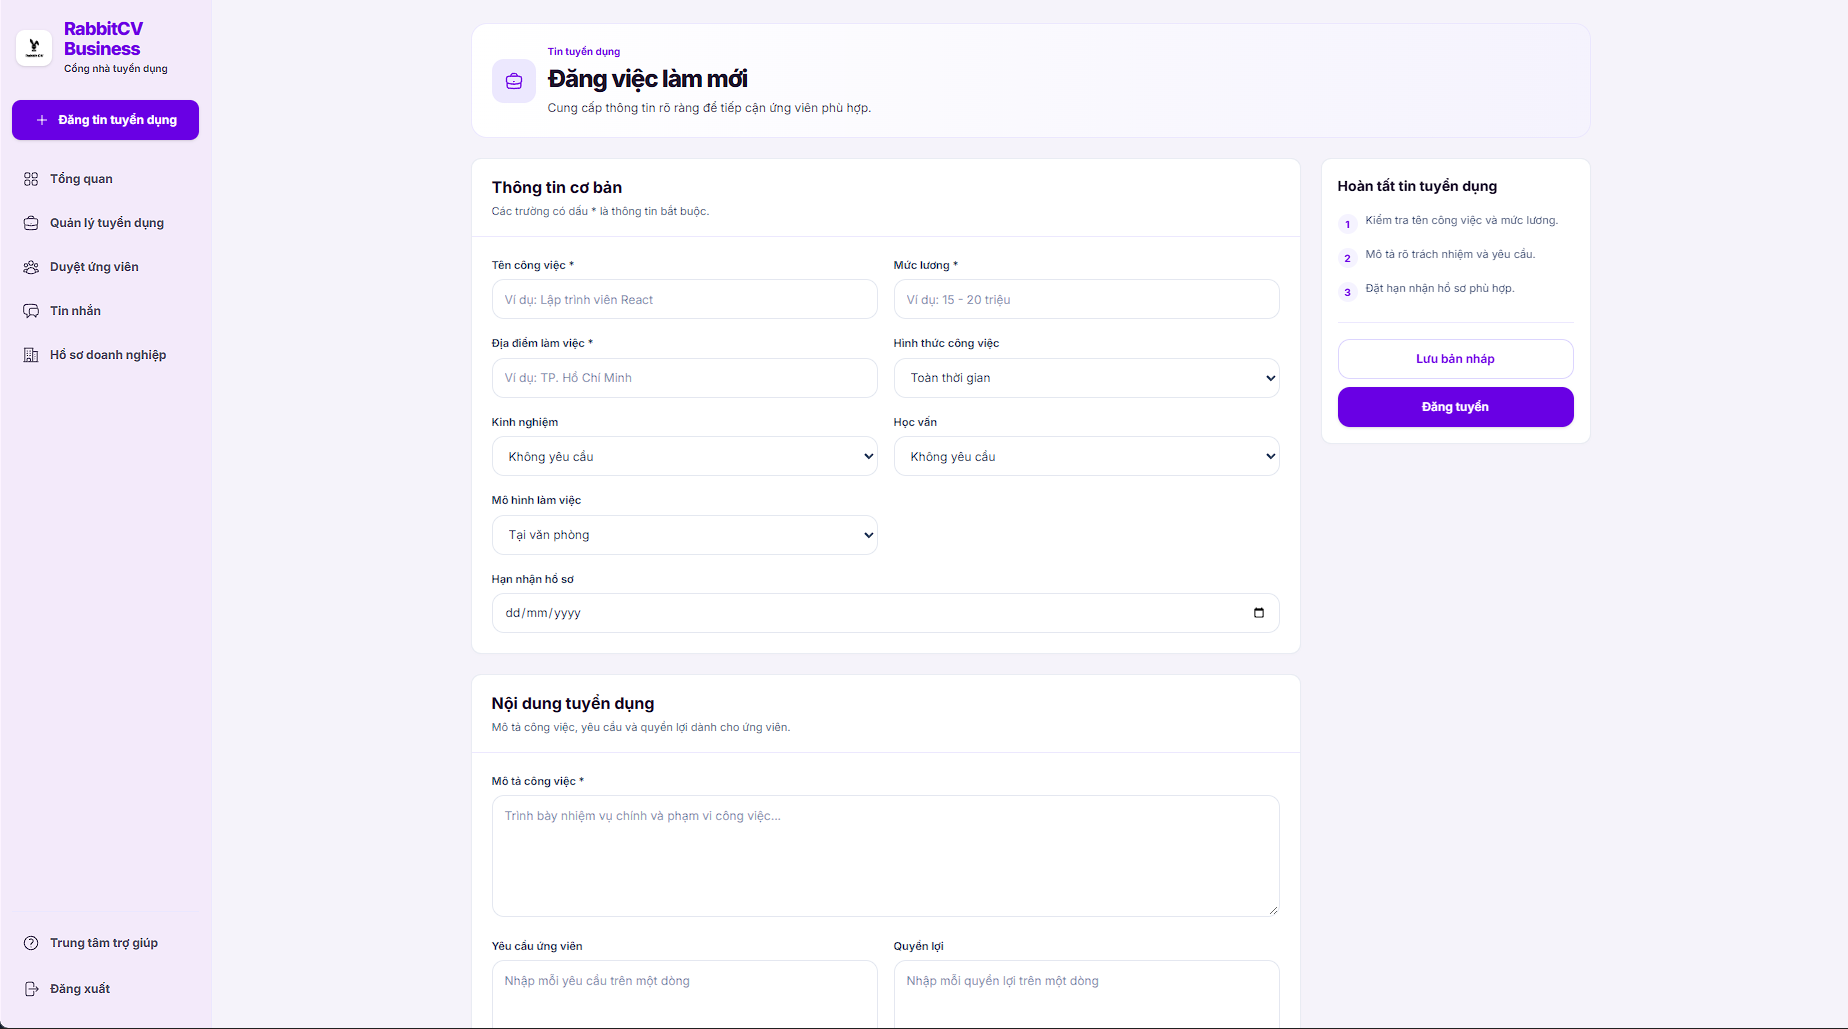
\includegraphics[width=1\linewidth,keepaspectratio]{img/CompanyJobPost.png}
    \caption{Giao diện đăng tin tuyển dụng mới}
    \label{fig:companyjobpost}
\end{figure}

Trang đăng tin tuyển dụng (Hình~\ref{fig:companyjobpost}) gồm thông tin vị trí, mức lương, địa điểm, hình thức và mô hình làm việc, kinh nghiệm, học vấn, thời hạn nhận hồ sơ, mô tả, yêu cầu và quyền lợi. Tài khoản doanh nghiệp phải được phê duyệt và không bị khóa mới có thể đăng tin. Người dùng có thể lưu nháp hoặc gửi đăng tuyển; doanh nghiệp đã xác minh được công khai tin theo chính sách hệ thống, còn doanh nghiệp chưa xác minh phải chờ quản trị viên duyệt tin.

Backend kiểm tra trạng thái tài khoản và dữ liệu tin, xác định trạng thái xét duyệt rồi lưu vào \texttt{Job}. Kết quả trả về giúp giao diện phân biệt tin đã lưu nháp, tin chờ duyệt và tin được công khai, thay vì thông báo mọi thao tác gửi đều là đăng tuyển thành công.

\subsection{Quản lý tuyển dụng}

\begin{figure}[H]
    \centering
    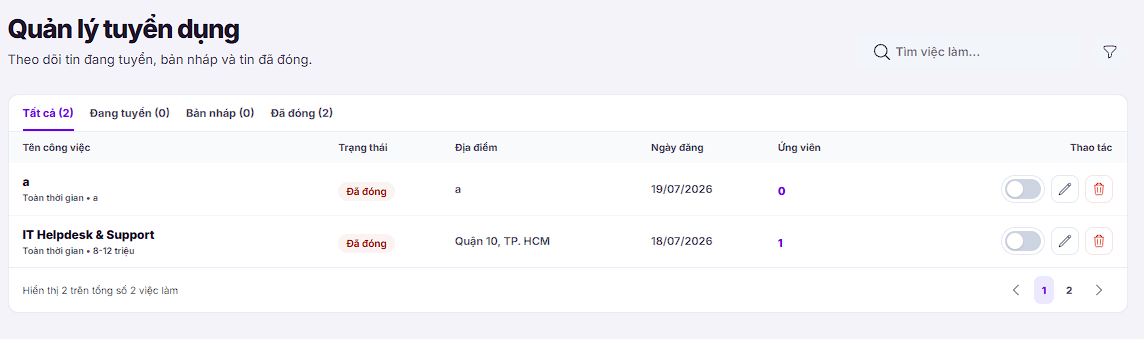
\includegraphics[width=1\linewidth,keepaspectratio]{img/CompanyJobManagement.png}
    \caption{Giao diện quản lý tin tuyển dụng}
    \label{fig:companyjobmanagement}
\end{figure}

Trang quản lý tuyển dụng (Hình~\ref{fig:companyjobmanagement}) hiển thị các tin thuộc doanh nghiệp theo trạng thái đang tuyển, bản nháp, chờ duyệt, không được duyệt và đã đóng. Mỗi tin có thông tin vị trí, địa điểm, ngày đăng và số hồ sơ đã tiếp nhận. Doanh nghiệp có thể chỉnh sửa nội dung, thay đổi thời hạn, đóng tin hoặc xóa tin trong phạm vi quyền sở hữu và điều kiện xét duyệt.

Thao tác xóa đánh dấu tin bằng trạng thái \texttt{Deleted} và thời điểm \texttt{deletedAt}, không xóa các hồ sơ ứng tuyển đã phát sinh. Nội dung sửa được xử lý lại theo chính sách xét duyệt của doanh nghiệp; tin bị quản trị viên ẩn không được tự động công khai lại chỉ bằng thao tác của doanh nghiệp.

\subsection{Duyệt ứng viên}

\begin{figure}[H]
    \centering
    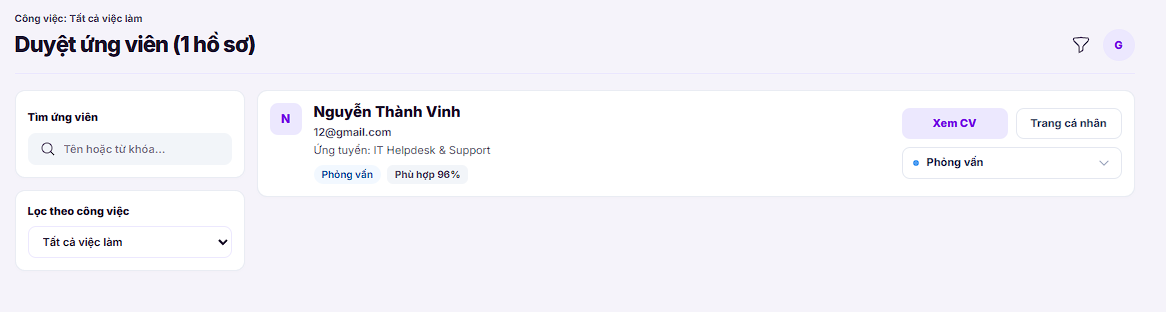
\includegraphics[width=1\linewidth,keepaspectratio]{img/CompanyReviewing.png}
    \caption{Giao diện duyệt hồ sơ ứng viên}
    \label{fig:companyreviewing}
\end{figure}

Trang duyệt ứng viên (Hình~\ref{fig:companyreviewing}) hỗ trợ tìm kiếm và lọc hồ sơ theo tin tuyển dụng, xem bản CV đã nộp và cập nhật trạng thái xử lý. Sáu trạng thái tương ứng là Chờ duyệt (\texttt{Pending}), Đang xem xét (\texttt{Reviewing}), Phỏng vấn (\texttt{Interview}), Đã đề nghị (\texttt{Offered}), Đã nhận (\texttt{Accepted}) và Từ chối (\texttt{Rejected}). Hồ sơ đã bị từ chối được khóa cập nhật trạng thái, thay vì chỉ ẩn lựa chọn trên giao diện.

Trang xem CV lấy dữ liệu theo mã hồ sơ ứng tuyển qua API riêng. Backend kiểm tra người gọi là chủ hồ sơ, doanh nghiệp sở hữu tin liên quan hoặc quản trị viên, rồi trả bản chụp CV để dựng bằng \texttt{ResumePreview} hoặc đọc bằng PDF.js. Đối với hồ sơ cũ chưa có bản chụp, hệ thống sử dụng phiên bản CV còn tồn tại và phân biệt nguồn bản chụp; không khẳng định đó là bản gốc lúc ứng tuyển. Việc đổi trạng thái hợp lệ được lưu tại backend và tạo thông báo cho ứng viên.

\subsection{Nhắn tin tuyển dụng}

\begin{figure}[H]
    \centering
    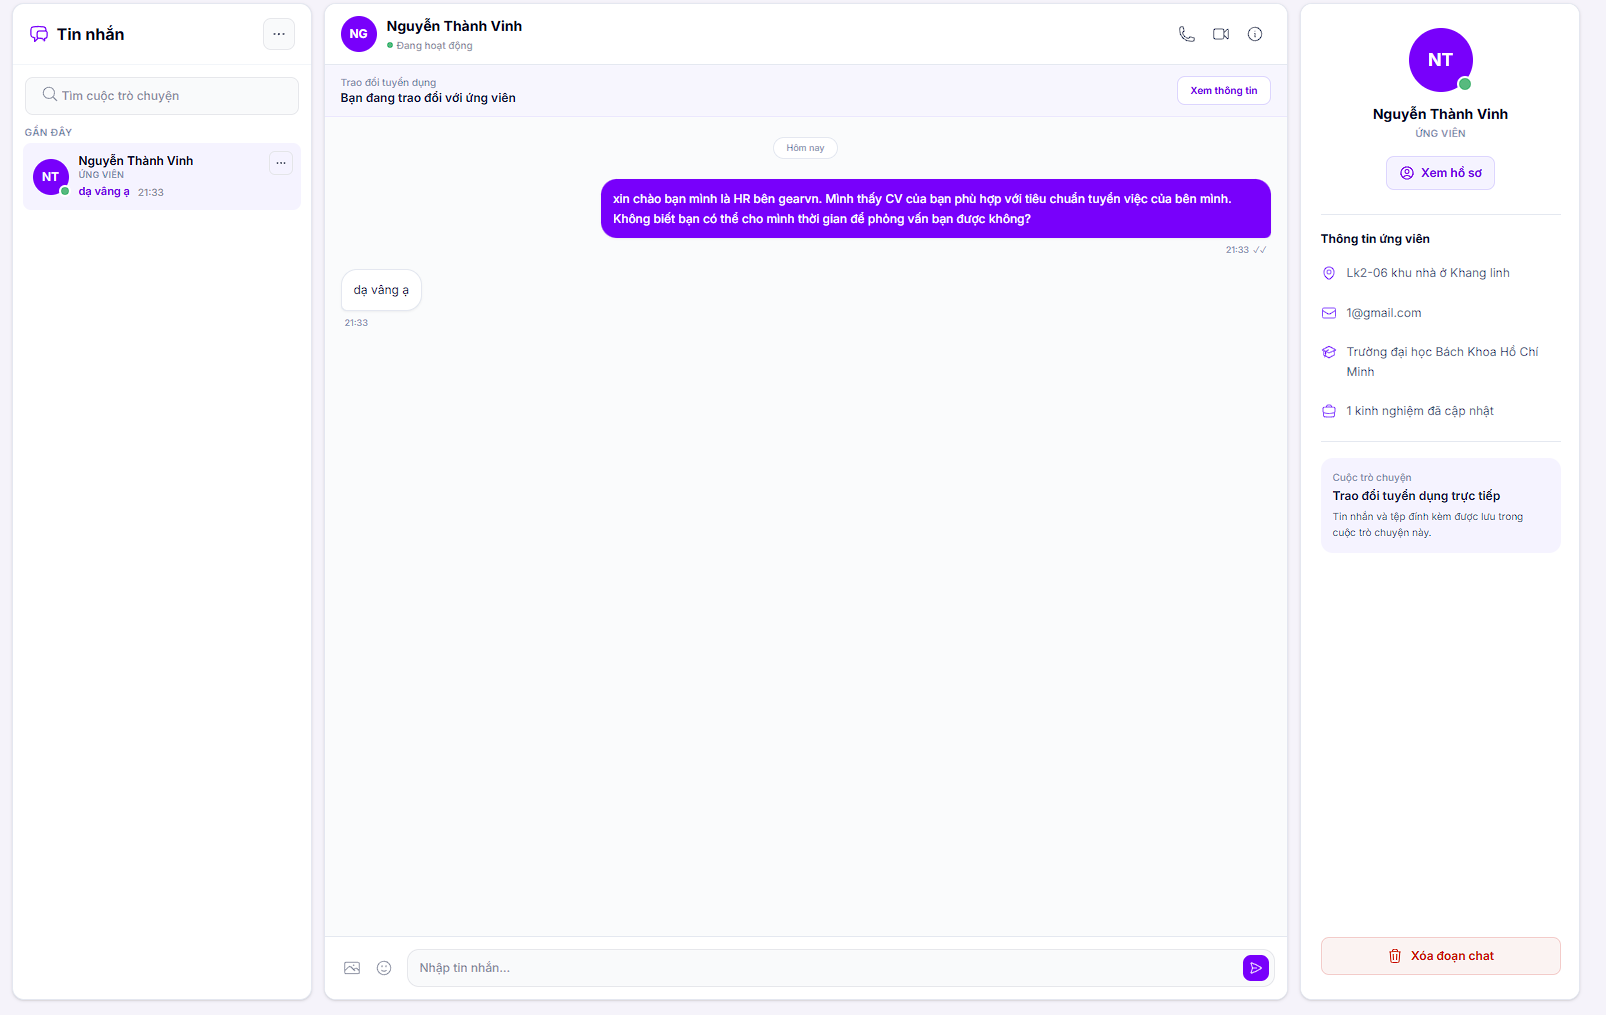
\includegraphics[width=1\linewidth,keepaspectratio]{img/CompanyChat.png}
    \caption{Giao diện nhắn tin trao đổi với ứng viên}
    \label{fig:companychat}
\end{figure}

Giao diện nhắn tin (Hình~\ref{fig:companychat}) cung cấp kênh trao đổi văn bản và hình ảnh giữa doanh nghiệp và ứng viên. Khung hội thoại hiển thị lịch sử, còn khu vực thông tin liên quan hỗ trợ xem hồ sơ người đang trao đổi. Hai bên có thể thỏa thuận thời gian phỏng vấn bằng tin nhắn; đây chưa phải chức năng tạo và quản lý lịch hẹn riêng.

Tin nhắn được gửi qua REST API, lưu vào \texttt{Message} rồi phát sự kiện \texttt{newMessage} đến phòng Socket.IO theo người nhận. Nếu người nhận chưa kết nối, nội dung vẫn có thể được tải lại từ lịch sử. \texttt{ChatReadState} lưu mốc đọc theo người dùng và hội thoại; \texttt{HiddenChat} lưu việc ẩn ở phía người thực hiện, không xóa tin nhắn của phía còn lại. Thông báo nghiệp vụ được lưu riêng và cập nhật qua sự kiện \texttt{newNotification} kết hợp truy vấn định kỳ mỗi 30 giây.


\section{Quản trị viên}

\subsection{Trang tổng quan}

\begin{figure}[H]
    \centering
    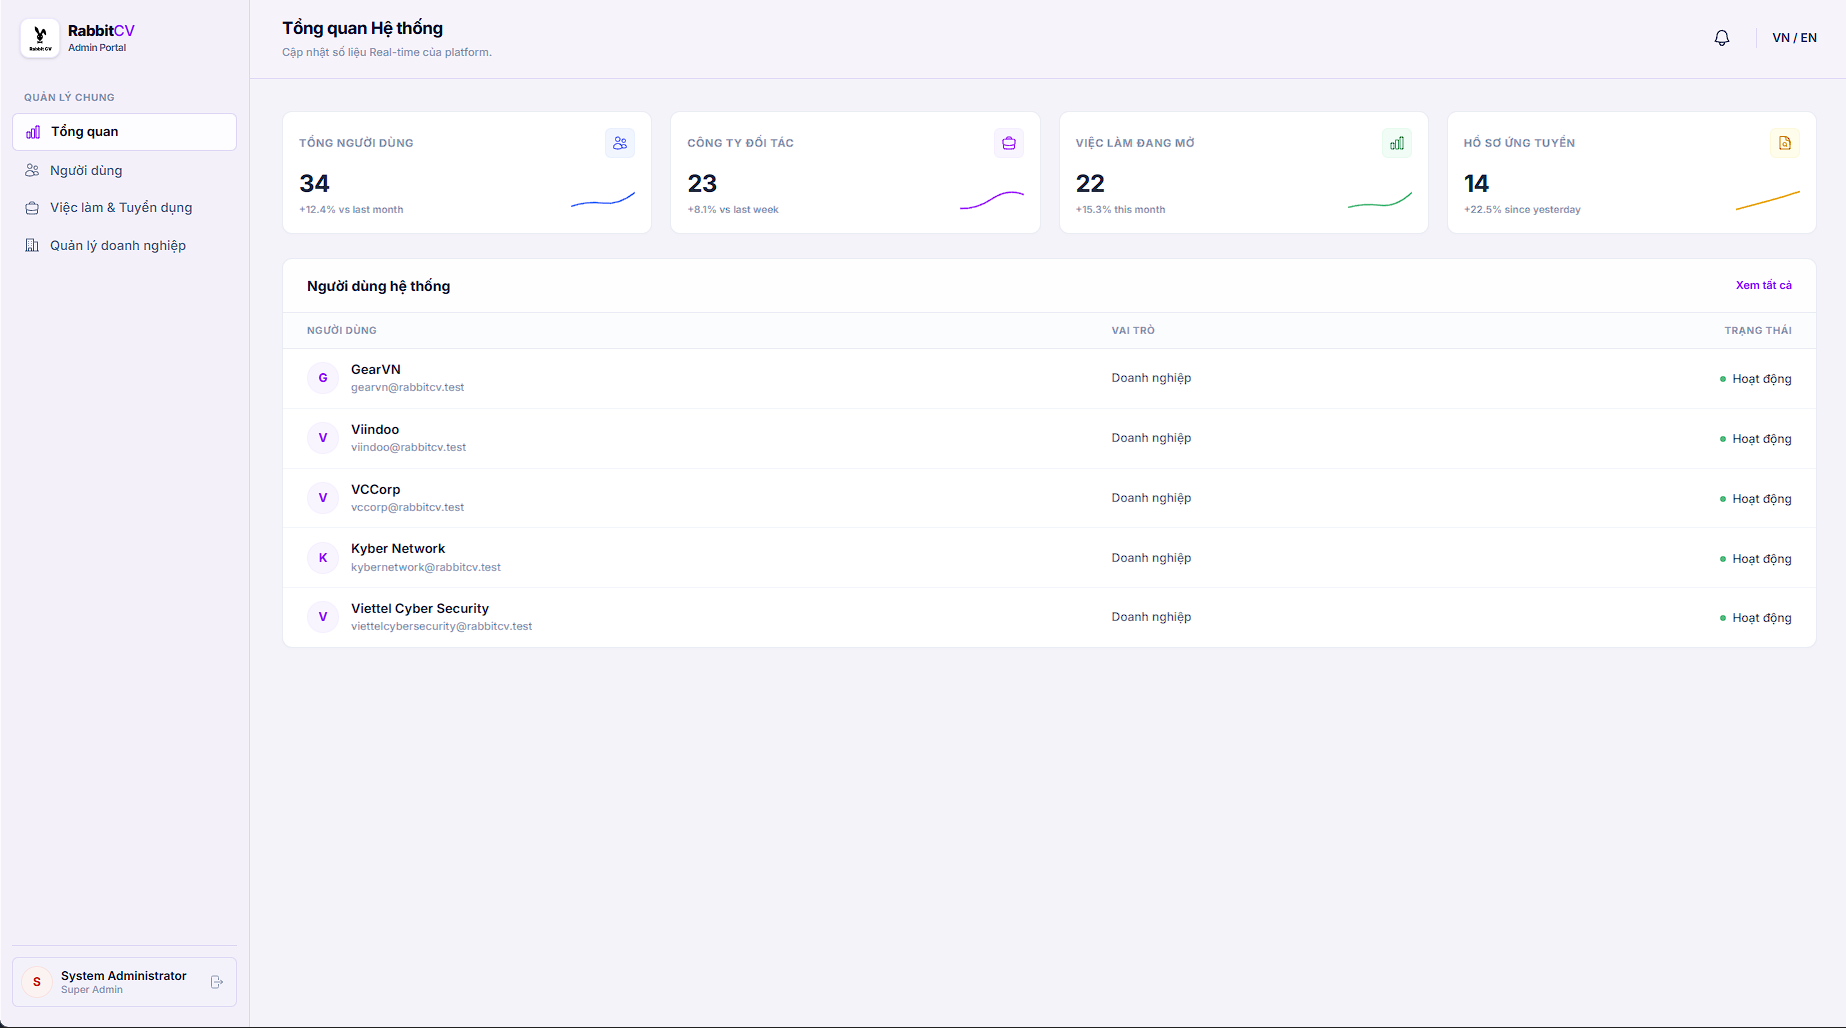
\includegraphics[width=0.9\linewidth,keepaspectratio]{img/AdminOverview.png}
    \caption{Giao diện tổng quan hệ thống dành cho quản trị viên}
    \label{fig:adminoverview}
\end{figure}

Trang tổng quan (Hình~\ref{fig:adminoverview}) hiển thị tổng số tài khoản chưa bị vô hiệu hóa, tài khoản doanh nghiệp, tin tuyển dụng chưa bị xóa mềm và hồ sơ ứng tuyển. Dữ liệu được lấy từ API thống kê khi trang được tải, không được cập nhật bằng cơ chế thời gian thực. Bảng người dùng phía dưới hiển thị thông tin tài khoản, vai trò và trạng thái.

Chỉ số \texttt{totalJobs} đếm tin chưa bị xóa mềm, không chỉ tin đang nhận hồ sơ; do đó nhãn \textit{``Việc làm đang mở''} trên giao diện chưa phản ánh đúng phạm vi dữ liệu. Các tỷ lệ tăng trưởng và đường xu hướng đang là dữ liệu trình diễn ở frontend, không phải kết quả so sánh thống kê theo thời gian.

\subsection{Quản lý người dùng}

\begin{figure}[H]
    \centering
    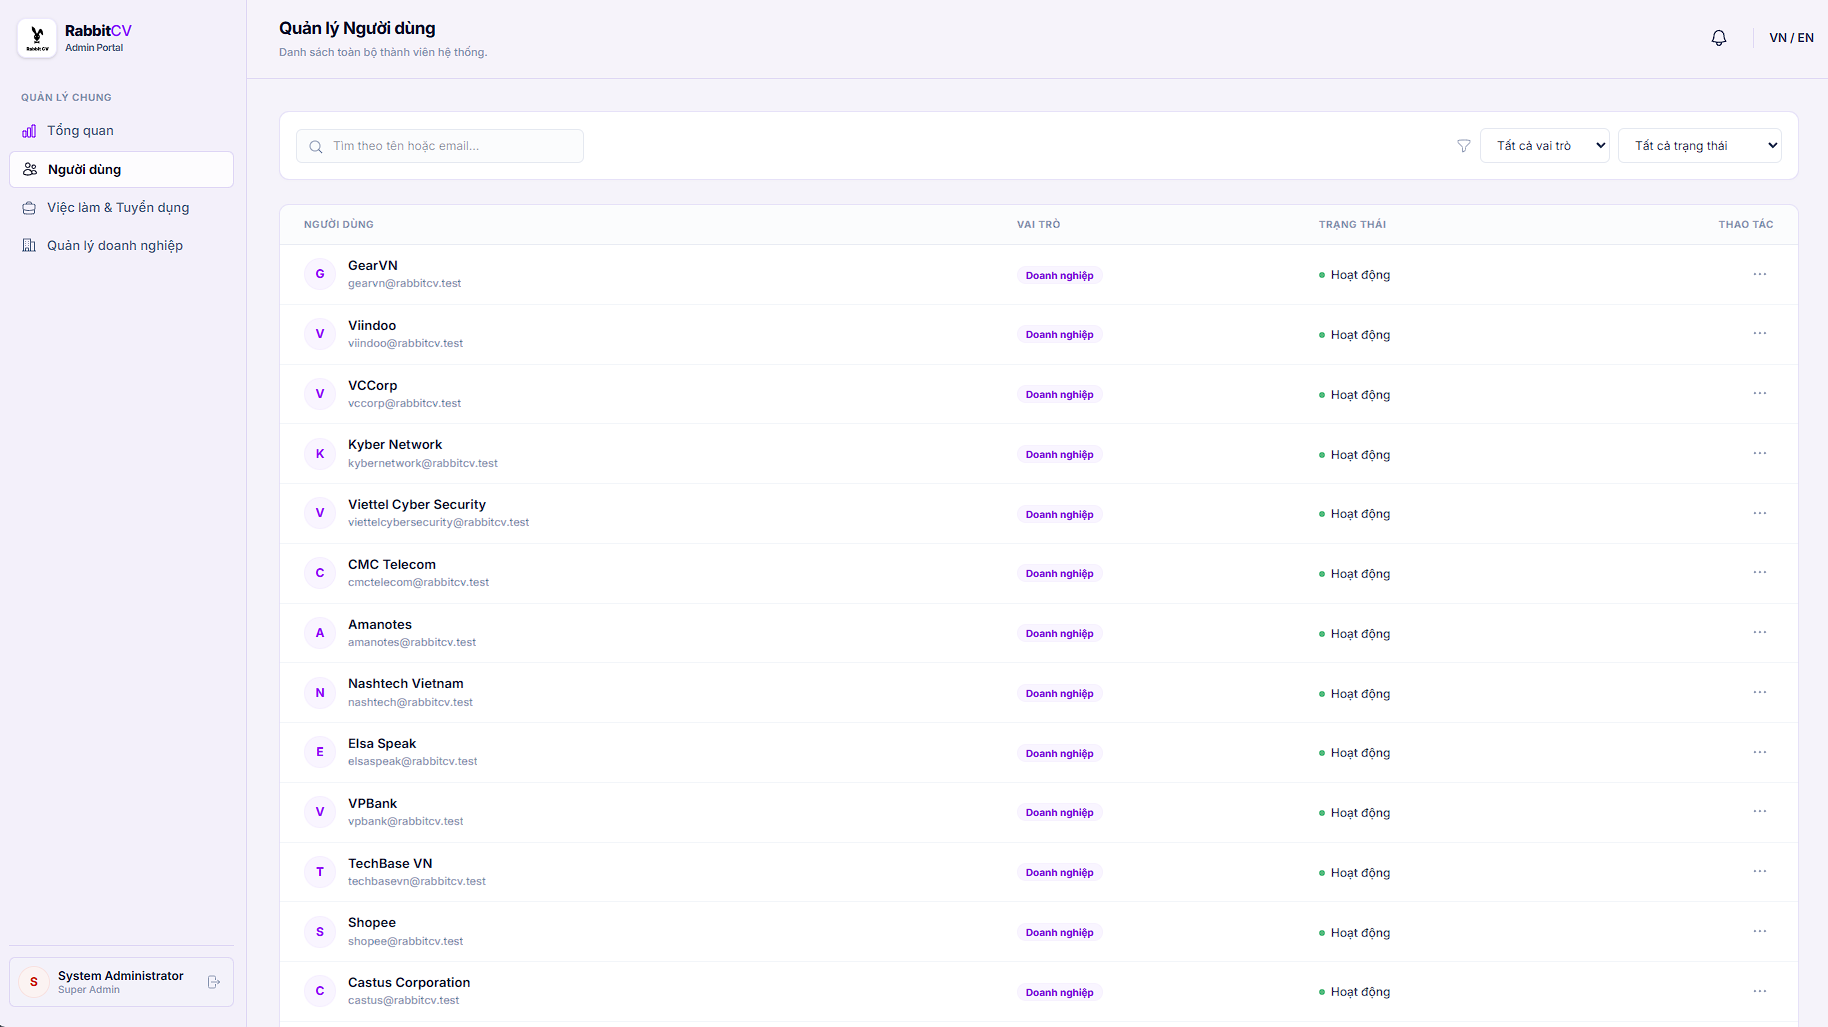
\includegraphics[width=0.9\linewidth,keepaspectratio]{img/UserManagement.png}
    \caption{Giao diện quản lý người dùng của quản trị viên}
    \label{fig:usermanagement}
\end{figure}

Trang quản lý người dùng (Hình~\ref{fig:usermanagement}) cho phép tìm tài khoản theo tên hoặc email và lọc theo vai trò, trạng thái. Các thao tác hiện có gồm khóa tài khoản và xóa theo cơ chế vô hiệu hóa; trang này chưa cung cấp mở khóa tài khoản người dùng thông thường. Backend không cho phép quản trị viên khóa hoặc xóa chính tài khoản đang sử dụng. Việc vô hiệu hóa tài khoản giữ lại lịch sử ứng tuyển; nếu là doanh nghiệp, các tin liên quan được gỡ khỏi danh sách công khai.

\subsection{Quản lý việc làm và tuyển dụng}

\begin{figure}[H]
    \centering
    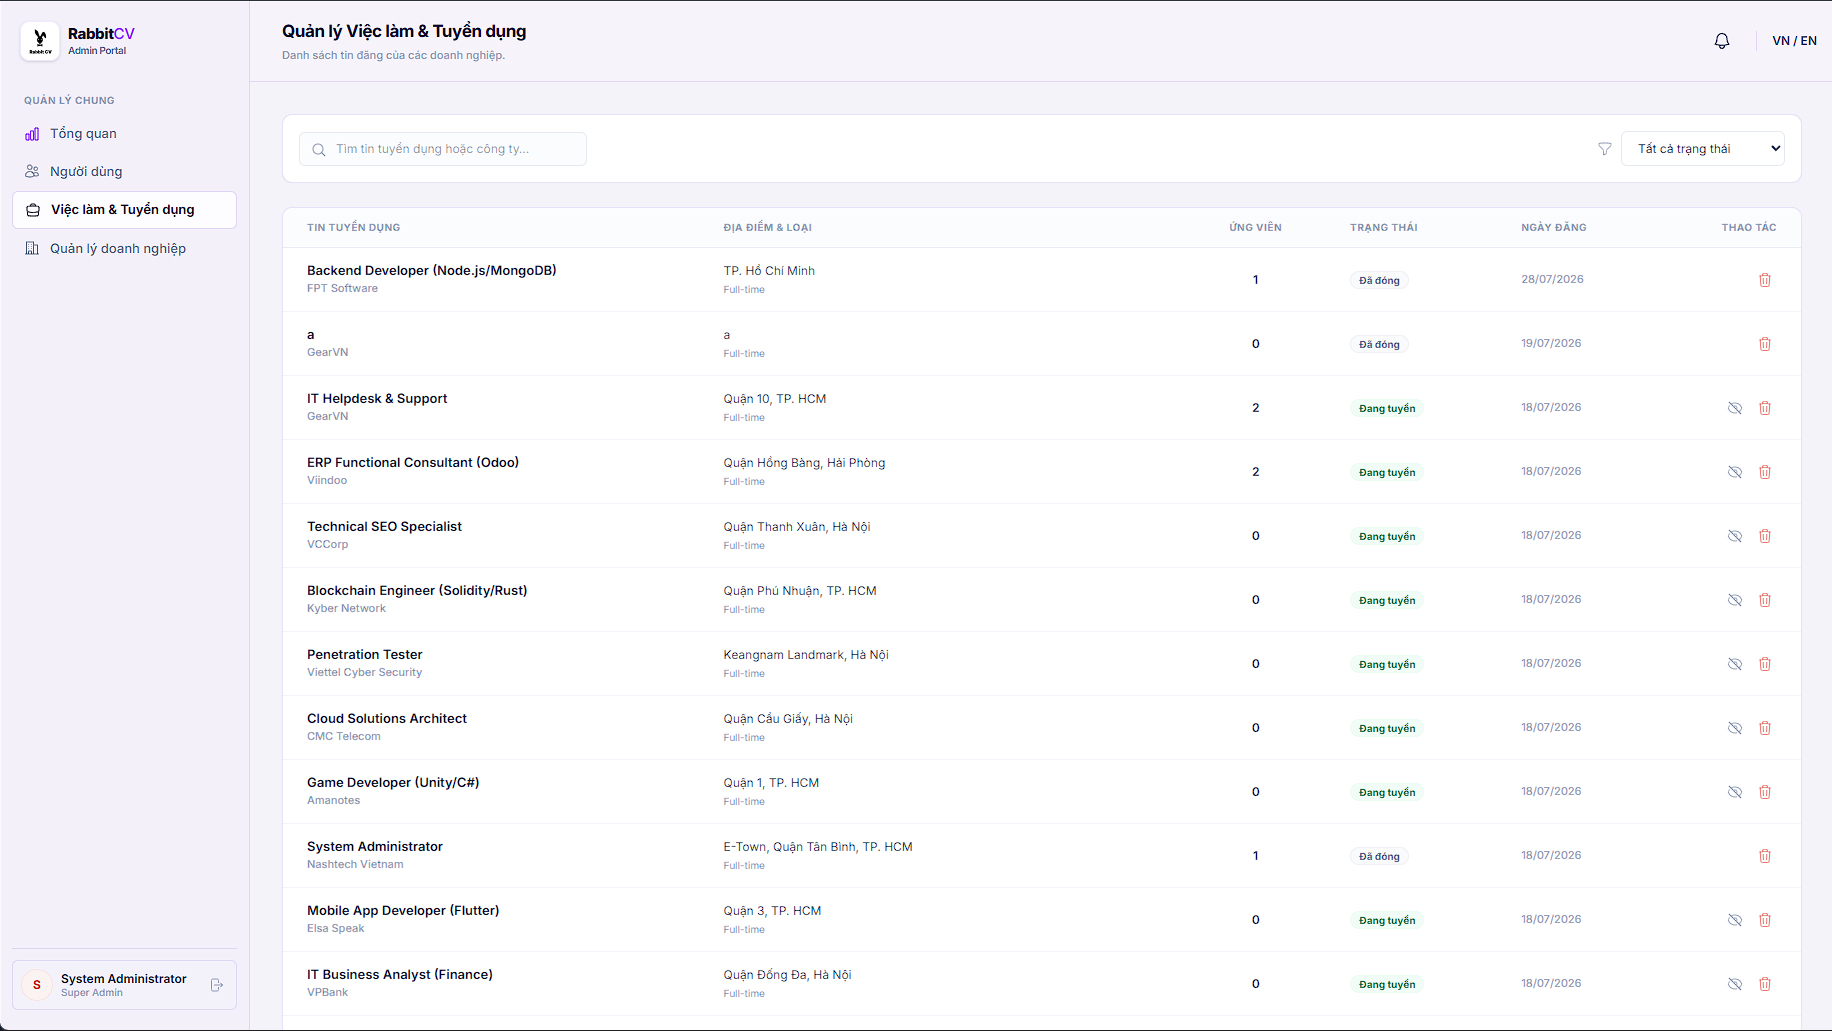
\includegraphics[width=0.9\linewidth,keepaspectratio]{img/JobManagement.png}
    \caption{Giao diện quản lý việc làm và tuyển dụng của quản trị viên}
    \label{fig:jobmanagement}
\end{figure}

Trang quản lý việc làm (Hình~\ref{fig:jobmanagement}) hỗ trợ tìm kiếm, lọc và xét duyệt tin của các doanh nghiệp. Quản trị viên có thể duyệt hoặc từ chối tin chờ xét duyệt, nhập lý do từ chối, ẩn hoặc hiển thị lại tin đã được duyệt và xóa mềm tin vi phạm. Những trạng thái này được phân biệt với bản nháp và tin đã đóng để tránh coi tin chờ duyệt là tin đang công khai.

Backend kiểm tra quyền quản trị và điều kiện thao tác trước khi cập nhật \texttt{Job}. Xét duyệt tin tạo thông báo kết quả cho doanh nghiệp; ẩn hoặc xóa mềm tin làm thay đổi khả năng truy cập công khai nhưng không xóa các hồ sơ ứng tuyển và bản chụp đã lưu.

\subsection{Quản lý doanh nghiệp}

\begin{figure}[H]
    \centering
    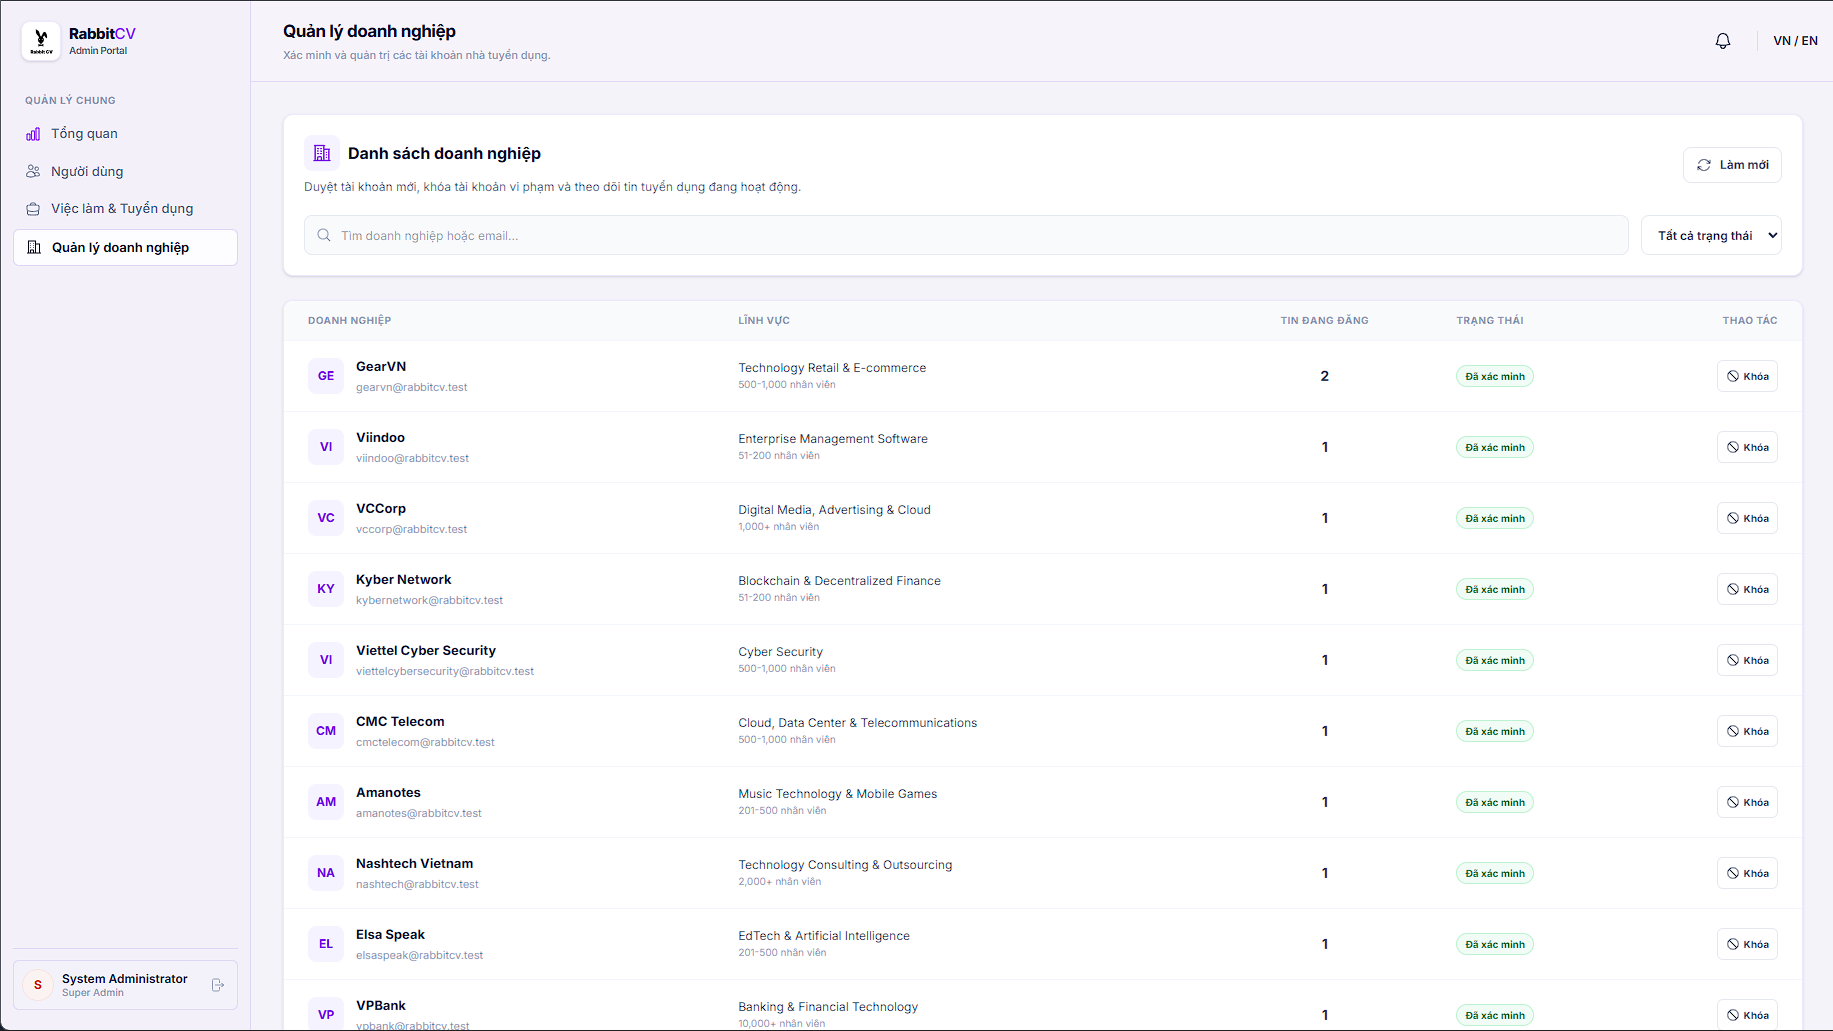
\includegraphics[width=0.9\linewidth,keepaspectratio]{img/CompanyManagement.png}
    \caption{Giao diện quản lý doanh nghiệp của quản trị viên}
    \label{fig:companymanagement}
\end{figure}

Trang quản lý doanh nghiệp (Hình~\ref{fig:companymanagement}) hiển thị danh sách và thông tin đăng ký để quản trị viên tạo tài khoản doanh nghiệp, phê duyệt hoặc từ chối tài khoản, xác minh hoặc thu hồi xác minh, khóa hoặc mở khóa. Khi từ chối tài khoản, quản trị viên phải cung cấp lý do; việc xác minh yêu cầu tài khoản đã được phê duyệt và không bị khóa.

Hai trạng thái phê duyệt tài khoản và xác minh doanh nghiệp được lưu riêng. Phê duyệt cho phép tài khoản sử dụng chức năng đăng tin, còn xác minh quyết định tin được công khai ngay hay phải chờ xét duyệt. Thao tác mở khóa ở khu vực này không đồng nghĩa trang quản lý người dùng đã có chức năng mở khóa chung cho mọi vai trò.


% \section{Tìm việc và ứng tuyển}

% Endpoint danh sách Job là tài nguyên công khai; giao diện hỗ trợ tìm từ khóa, công ty, địa điểm và thẻ, đồng thời phân biệt trạng thái tin. Với người dùng đã đăng nhập, SavedJobsContext giữ giao diện dùng chung nhưng dữ liệu được quản lý bằng TanStack Query. Thao tác lưu/bỏ lưu cập nhật cache lạc quan, khôi phục trạng thái cũ khi API thất bại và làm mới lại sau khi hoàn tất.

% \begin{figure}[H]
%     \centering
%     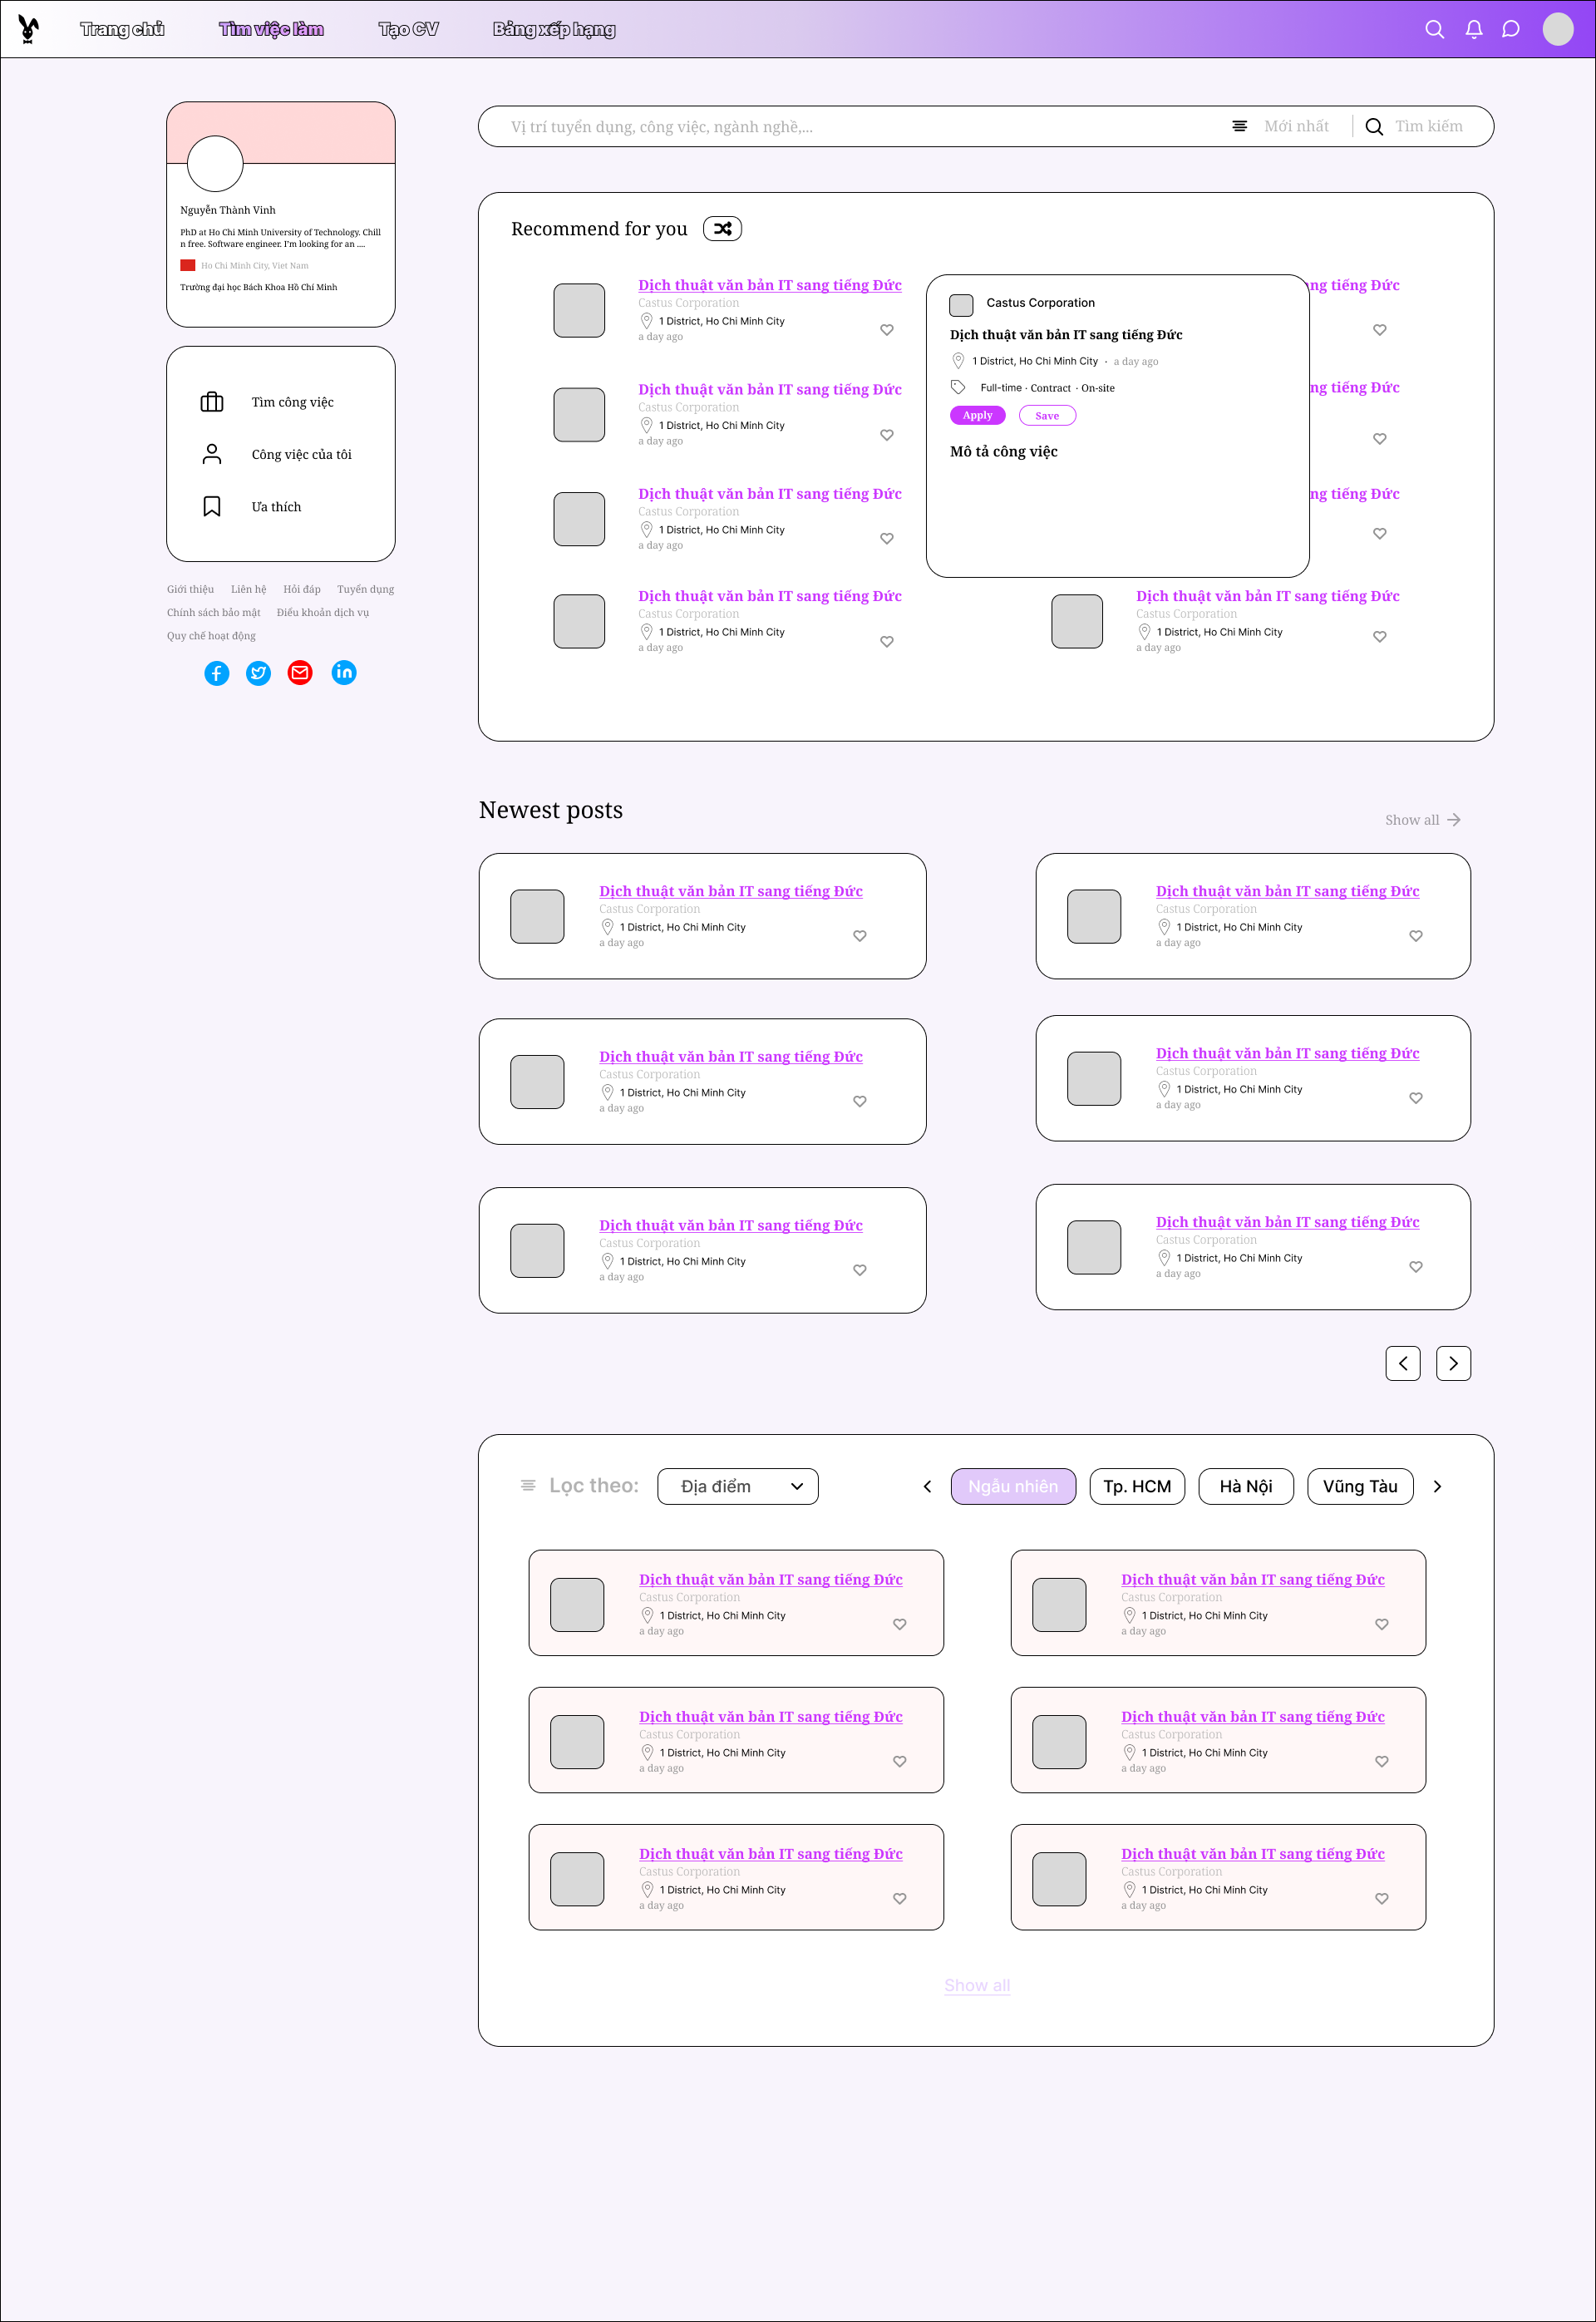
\includegraphics[height=0.58\textheight,trim=0 560 0 0,clip]{img/FindingJob.png}
%     \caption{Giao diện tìm kiếm và xem nhanh việc làm}
%     \label{fig:finding-job}
% \end{figure}

% Người dùng đã xác thực có thể nộp Resume đã lưu hoặc tải một PDF mới qua hai endpoint ứng tuyển tương ứng. Trước khi ghi dữ liệu, backend xác nhận tài khoản, quyền sở hữu CV, trạng thái và hạn của Job. Unique index trên cặp \texttt{jobId}--\texttt{candidateId} là lớp bảo vệ cuối cùng chống ứng tuyển trùng, kể cả khi hai request đến gần nhau. API hiện chưa kiểm tra rõ vai trò phải là ứng viên; đây là điểm cần hoàn thiện thay vì chỉ dựa vào điều hướng frontend.

% Application lưu \texttt{jobSnapshot} gồm các thông tin cần thiết của tin tại thời điểm nộp. Nhờ đó, lịch sử ứng tuyển vẫn có ngữ cảnh nếu doanh nghiệp xóa Job. Với PDF upload hợp lệ, backend tạo Resume ảo và liên kết với Application; Resume này không xuất hiện trong danh sách CV quản lý thường ngày.

% \section{Cổng doanh nghiệp}

% Doanh nghiệp dùng chung cơ chế xác thực nhưng có bố cục và route riêng. Các chức năng đã triển khai gồm:

% \begin{itemize}
%     \item cập nhật hồ sơ công ty;
%     \item tạo tin nháp, đăng hoặc chỉnh sửa tin;
%     \item bật hoặc tắt nhận hồ sơ và xóa tin;
%     \item xem danh sách ứng viên;
%     \item cập nhật trạng thái Application.
% \end{itemize}

% Trạng thái hồ sơ gồm Pending, Reviewing, Interview, Offered, Rejected và Accepted. Form tin tuyển dụng bổ sung kinh nghiệm, học vấn, mô hình làm việc và kiểm tra hạn tối đa hai năm. Tuy nhiên, trạng thái xác minh doanh nghiệp chưa được kiểm tra tại endpoint tạo tin, nên quy trình duyệt chưa phải một cổng cưỡng chế hoàn chỉnh.

% Khi doanh nghiệp yêu cầu xem CV, backend không chỉ kiểm tra role company mà còn kiểm tra Job/Application liên quan. Khi trạng thái Application thay đổi, hệ thống tạo Notification cho ứng viên. Cơ chế này liên kết thao tác tuyển dụng với lịch sử và thông báo, thay vì để từng màn hình thay đổi dữ liệu độc lập.

% \section{Chat và thông báo}

% Chat sử dụng mô hình ``lưu trước, phát sau''. Client gửi nội dung qua REST API; backend lấy danh tính người gửi từ JWT, kiểm tra có văn bản hoặc ảnh, lưu Message rồi phát sự kiện \texttt{newMessage} đến phòng của người nhận bằng Socket.IO. Nếu ghi cơ sở dữ liệu thất bại, server không phát một thông điệp chưa tồn tại. Văn bản được React hiển thị như chuỗi; ảnh được CompressorJS nén ở client trước khi chuyển thành data URL. Backend hiện chưa áp dụng giới hạn loại/dung lượng ảnh và chưa xác minh đầy đủ người gửi thuộc phòng riêng, vì vậy không gọi đây là luồng đã được làm sạch hoàn toàn.

% ChatReadState lưu \texttt{lastReadAt} theo người dùng và phòng để chỉ báo chưa đọc tồn tại qua lần tải lại. HiddenChat cho phép một người ẩn cuộc hội thoại khỏi danh sách của mình mà không xóa Message của phía còn lại; tin mới sau mốc ẩn có thể làm phòng xuất hiện lại. Notification là collection riêng, hỗ trợ phân trang, đếm chưa đọc, đánh dấu từng mục hoặc tất cả và xóa. Hook thông báo dùng TanStack Query để cache các trang, cập nhật trạng thái đọc trước trên giao diện và truy vấn số chưa đọc mỗi 30 giây; message dùng kết nối thời gian thực.

% \section{Khu vực quản trị}

% Backend cung cấp các nhóm chức năng quản trị sau:

% \begin{itemize}
%     \item thống kê và chẩn đoán health chi tiết;
%     \item xem danh sách, ẩn, hiện hoặc xóa Job;
%     \item xem danh sách và xác minh doanh nghiệp;
%     \item khóa hoặc xóa User.
% \end{itemize}

% Các endpoint này dùng xác thực và kiểm tra vai trò admin. Frontend hiện chỉ giữ các màn hình có API thật gồm dashboard, người dùng, việc làm và doanh nghiệp; các đường dẫn báo cáo, đánh giá và nhật ký cũ chuyển về trang hợp lệ. Endpoint khóa User hiện chỉ đặt trạng thái khóa, chưa có thao tác mở lại tương ứng cho tài khoản thông thường. Vì vậy báo cáo ghi nhận quản trị ở mức cơ bản, không xem toàn bộ khu vực admin là hoàn tất.

% \section{Bảo mật và giới hạn triển khai}

% Các lớp bảo vệ chính trong quá trình triển khai gồm:

% \begin{itemize}
%     \item \textbf{HTTP header:} Helmet thiết lập CSP, chặn nhúng trang và đặt chính sách referrer; cấu hình Vercel bổ sung các header về quyền truy cập thiết bị, kiểu nội dung và tài nguyên chéo nguồn.
%     \item \textbf{Nguồn truy cập và tần suất:} CORS chỉ cho các origin được cấu hình; API chung chịu giới hạn 300 yêu cầu trong 15 phút, đăng nhập tối đa 10 lần thất bại trong 15 phút, đăng ký tối đa 10 lần mỗi giờ và AI có giới hạn riêng.
%     \item \textbf{Dữ liệu phản hồi:} các danh sách trường \texttt{SELF\_USER\_FIELDS}, \texttt{PUBLIC\_USER\_FIELDS} và \texttt{ADMIN\_USER\_FIELDS} giới hạn dữ liệu tài khoản được trả theo từng ngữ cảnh; mật khẩu và mã PIN không được đưa vào phản hồi.
% \end{itemize}

% Các biện pháp trên là lớp bảo vệ cơ bản, chưa phải chứng nhận an toàn. Khi thiếu biến môi trường, mã nguồn vẫn có khóa JWT dự phòng; kết nối cơ sở dữ liệu còn tự tạo tài khoản quản trị trình diễn với mật khẩu ngắn. Hai hành vi này thuận tiện cho phát triển nhưng không phù hợp production. Ngoài ra cần hoàn thiện kiểm tra vai trò cho AI/ứng tuyển/lưu việc, xác minh thành viên phòng chat ở mọi thao tác, CSRF, chính sách mật khẩu, giới hạn ảnh, nhật ký kiểm toán và quy trình xoay bí mật.
